% Created 2023-04-21 Fri 09:51
% Intended LaTeX compiler: pdflatex
\documentclass[11pt]{article}
\usepackage[utf8]{inputenc}
\usepackage[T1]{fontenc}
\usepackage{graphicx}
\usepackage{longtable}
\usepackage{wrapfig}
\usepackage{rotating}
\usepackage[normalem]{ulem}
\usepackage{amsmath}
\usepackage{amssymb}
\usepackage{capt-of}
\usepackage{hyperref}
\author{Jay Paul Morgan}
\date{\textit{<2023-04-21 Fri>}}
\title{MCH2023 - A retrospective}
\hypersetup{
 pdfauthor={Jay Paul Morgan},
 pdftitle={MCH2023 - A retrospective},
 pdfkeywords={},
 pdfsubject={},
 pdfcreator={Emacs 29.0.60 (Org mode 9.6.1)}, 
 pdflang={English}}
\begin{document}

\maketitle
\tableofcontents

\begin{figure}[htbp]
\centering
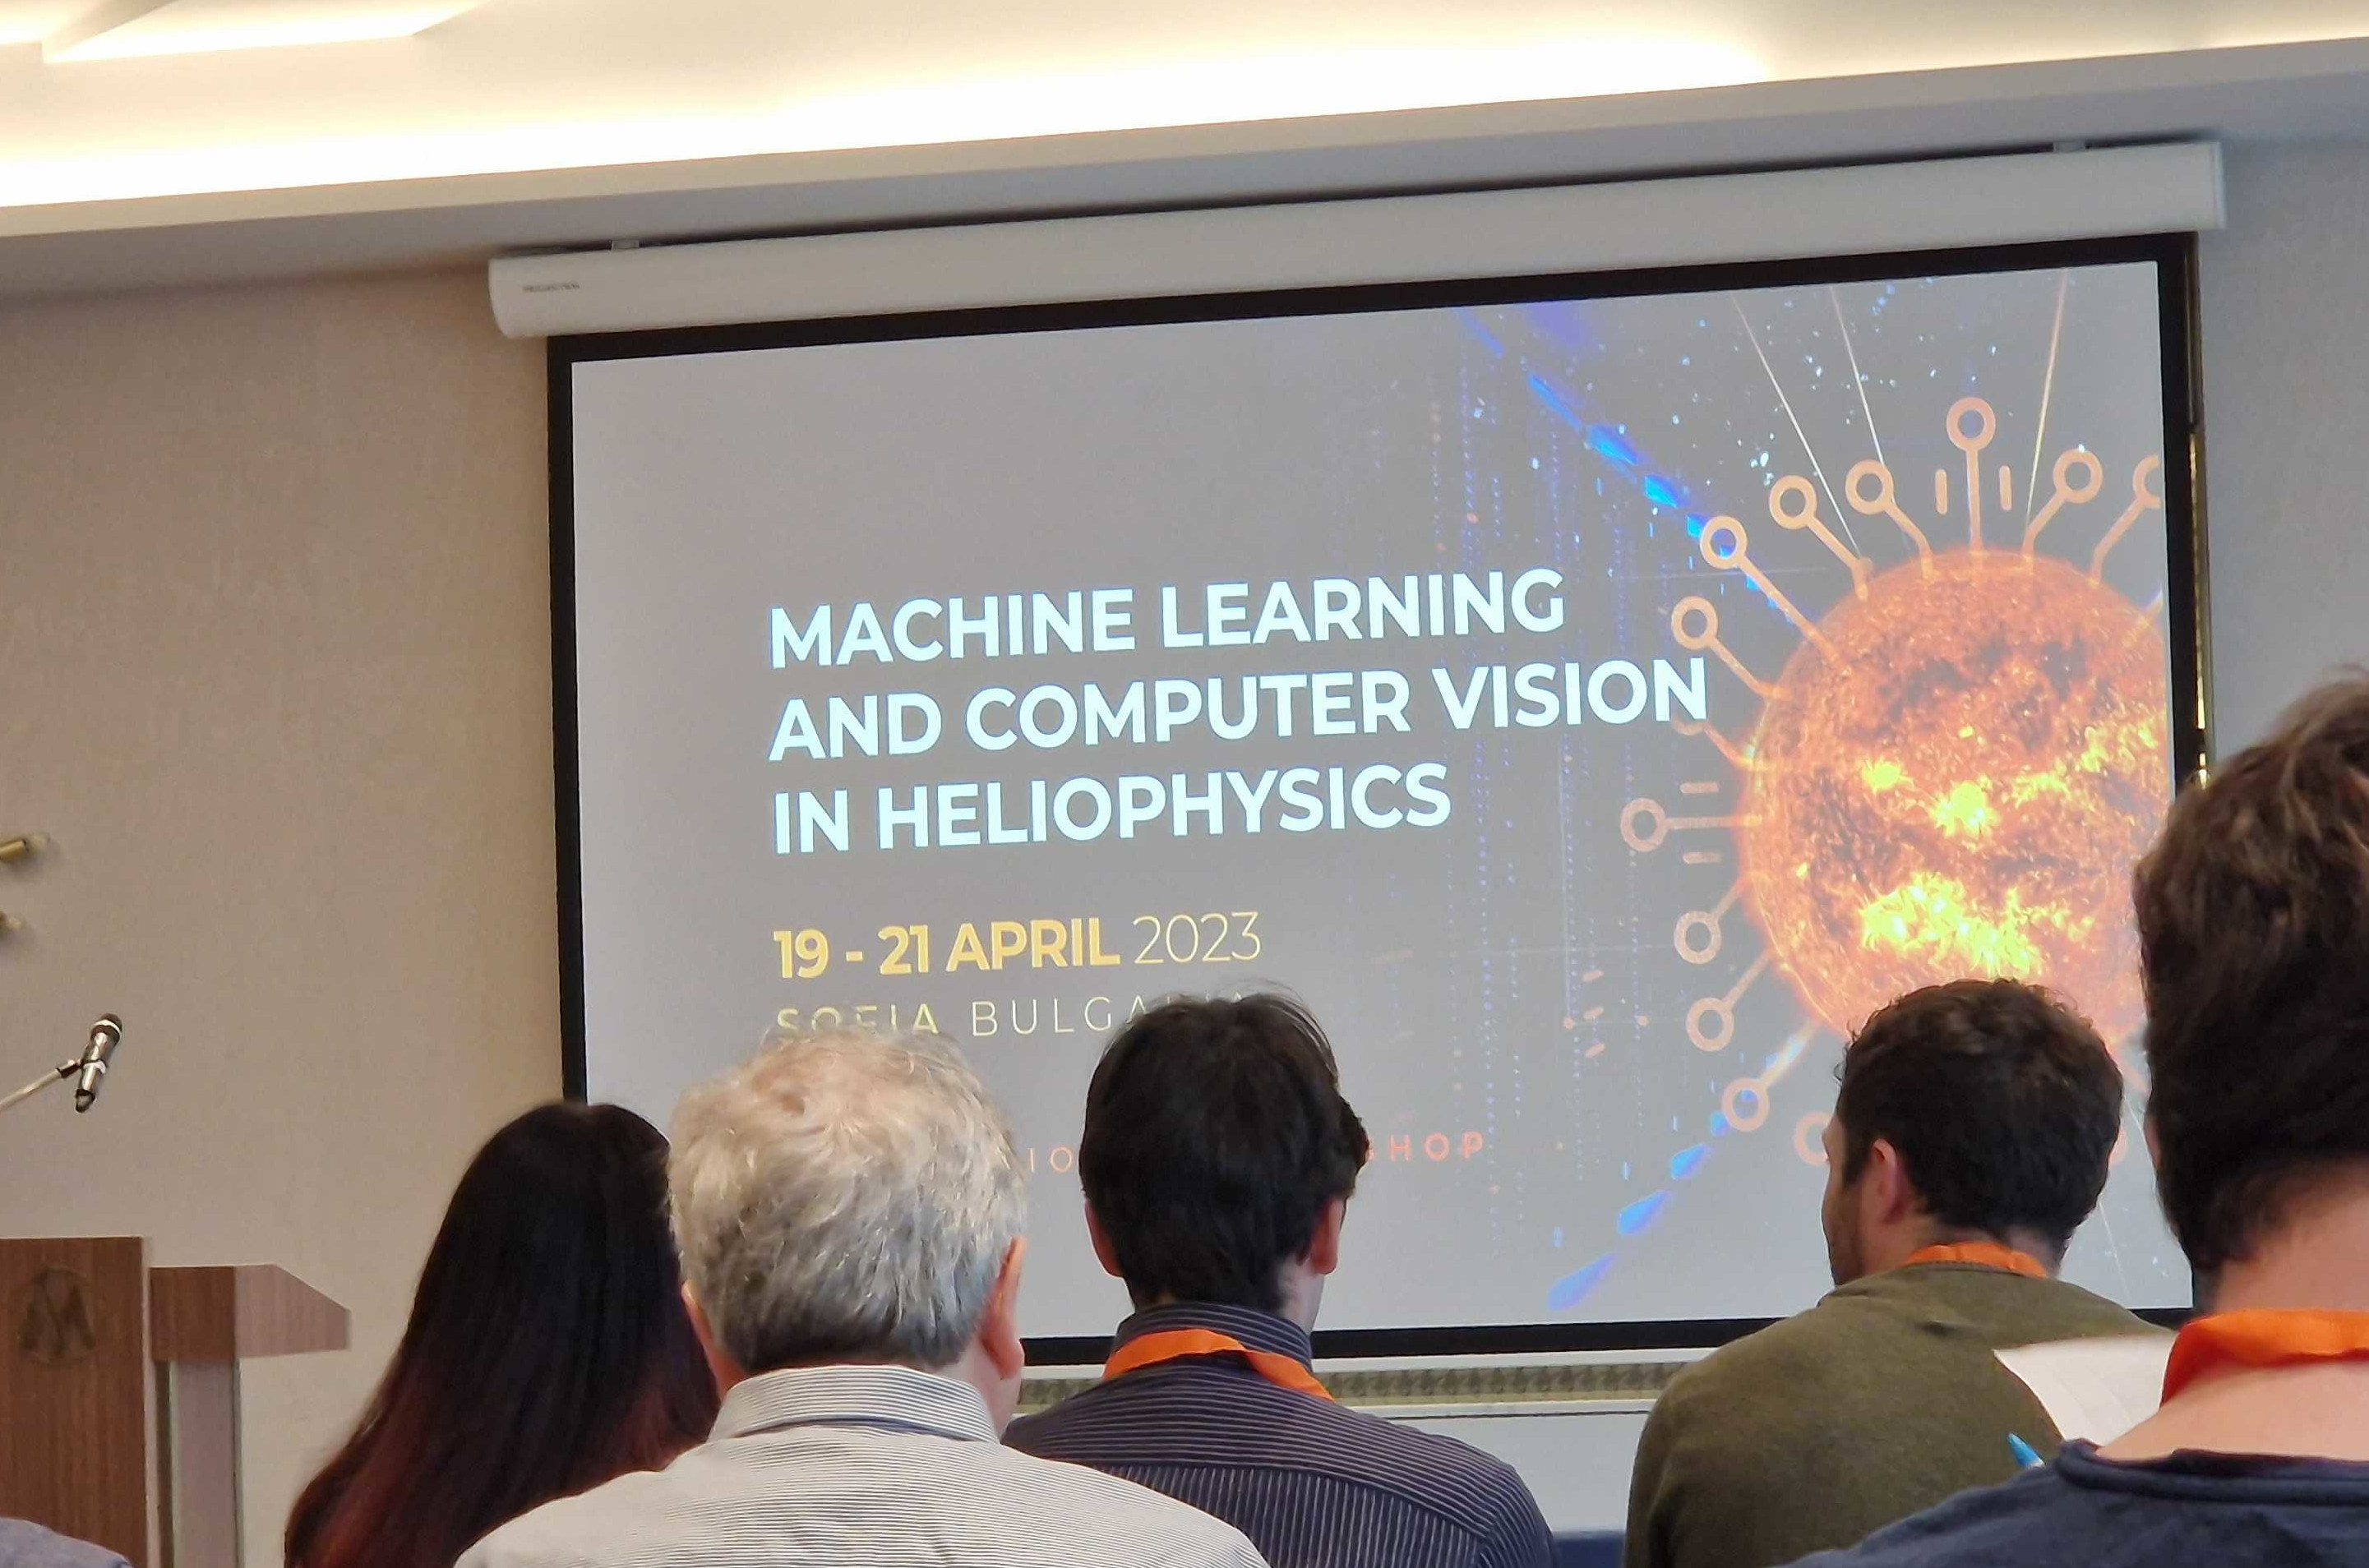
\includegraphics[width=1.0\textwidth]{images/20230419_085440.jpg}
\caption{2023 Machine Learning and Computer Vision in Heliophyics conference introduction.}
\end{figure}

The 2023 Machine Learning and Computer Vision in Heliophysics
conference, hosted in the luxurious Millennium hotel, Sofia, Bulgaria,
has now concluded after 3 days of interesting and thought-provoking
lectures.

Following this conference, I wanted to highlight some of the talks, as
well as drawing and picking up common threads that were interwoven
through all the presentations. From this, I hope to better understand
what the current research is, more than one would gain for looking at
each work in its isolation.

For a full list of the conference program, you can find it here.

If you were at this conference and you think that I've missed
something that should be covered in this discussion, please do get in
touch and let me know!

\section{Simple models are useful models}
\label{sec:org44dbf62}

While much of the work shows that thoughtful feature extraction,
coupled with domain knowledge, and selection of traditional machine
learning models can still produce reliable models upon which to make
predictions. Take for example, Hanne's talk where active regions are
classified using the magnetic properties. A small number of features
were selected by evaluating the usefulness and duplication of
information present in all the features. After a sparse autoencoder
was used to encode a slightly larger representation, that was
classified using a \$k\$-NN model in a supervised way, and \$k\$-means in
a unsupervised way.

But while, we have seen such use of traditional machine learning, Deep
Neural Networks (DNNs) are also used. I noticed a use of common models
through applications. In particular, we saw many applications feature
either U-Net or YOLO.

A. Denerke created a labelled (the labels being bounding-boxes)
dataset of filaments in the H-\(\alpha\) wavelength. These labels were
used to train a YOLO model to learn to recognise the presence of
filaments so that other, more computationally expensive algorithms,
could be used to create segmentation masks.

While YOLO was only used for object detection and segmentation (for
example \ldots{}), U-Net was also commonly used for segmentation, as well
as data generation in a GAN architecture, such as in the applications:

\begin{itemize}
\item \ldots{}
\item 
\end{itemize}

\section{More data is better data}
\label{sec:org6099f27}

Heliophyics is no exception in the world where more data is needed to
adequately train ML models. Despite many satellites, telescopes, and
other sensoring equipment constantly gathering data, a very large
percentage of the data being recorded contains nothing
interesting. For example, take Allin's talk in which they would like
to classify whether, based on a small number of features, a cosmic
mass ejection (CME) will interact with the Earth (geoeffective). In
this talk, 99.3\% of all data is non-geoeffective. Class-imbalance is
then a persistent problem. The disruptive events we want to detect and
predict happen very rarely.

In Vanessa's talk on the detection of sunquakes, these type of events
only happen around 2 times per year. Given then length of time since
they've been discovered, we haven't observed a whole lot of them.

The Synthetic Minority \ldots{} (SMOTE) algorithm was very often used to
generate synthetic examples of the rare positive cases.

In other cases, DNNs where used in a variety of ways. Firstly, we see
their use for synthetic data generation. Fransisco demonstrated a very
interesting method of generating solar disk images that contain
desired solar features using a Diffusion Probabilistic Model (DDPM).

Juan used a GAN architecture to generate stokes parameters.

As the events we're interested in happen very infrequently, but we're
recording all of the time, we are essentially wasting our storage with
useless data. Pierce used a U-Net trained to segment type-II and
type-III solar bursts so that data could be automatically binned and
we reduce the storage costs by restricting the saving data closer to
solar events.

Jeremiah cleaning of radio frequency interference using GANs.

\begin{figure}[htbp]
\centering
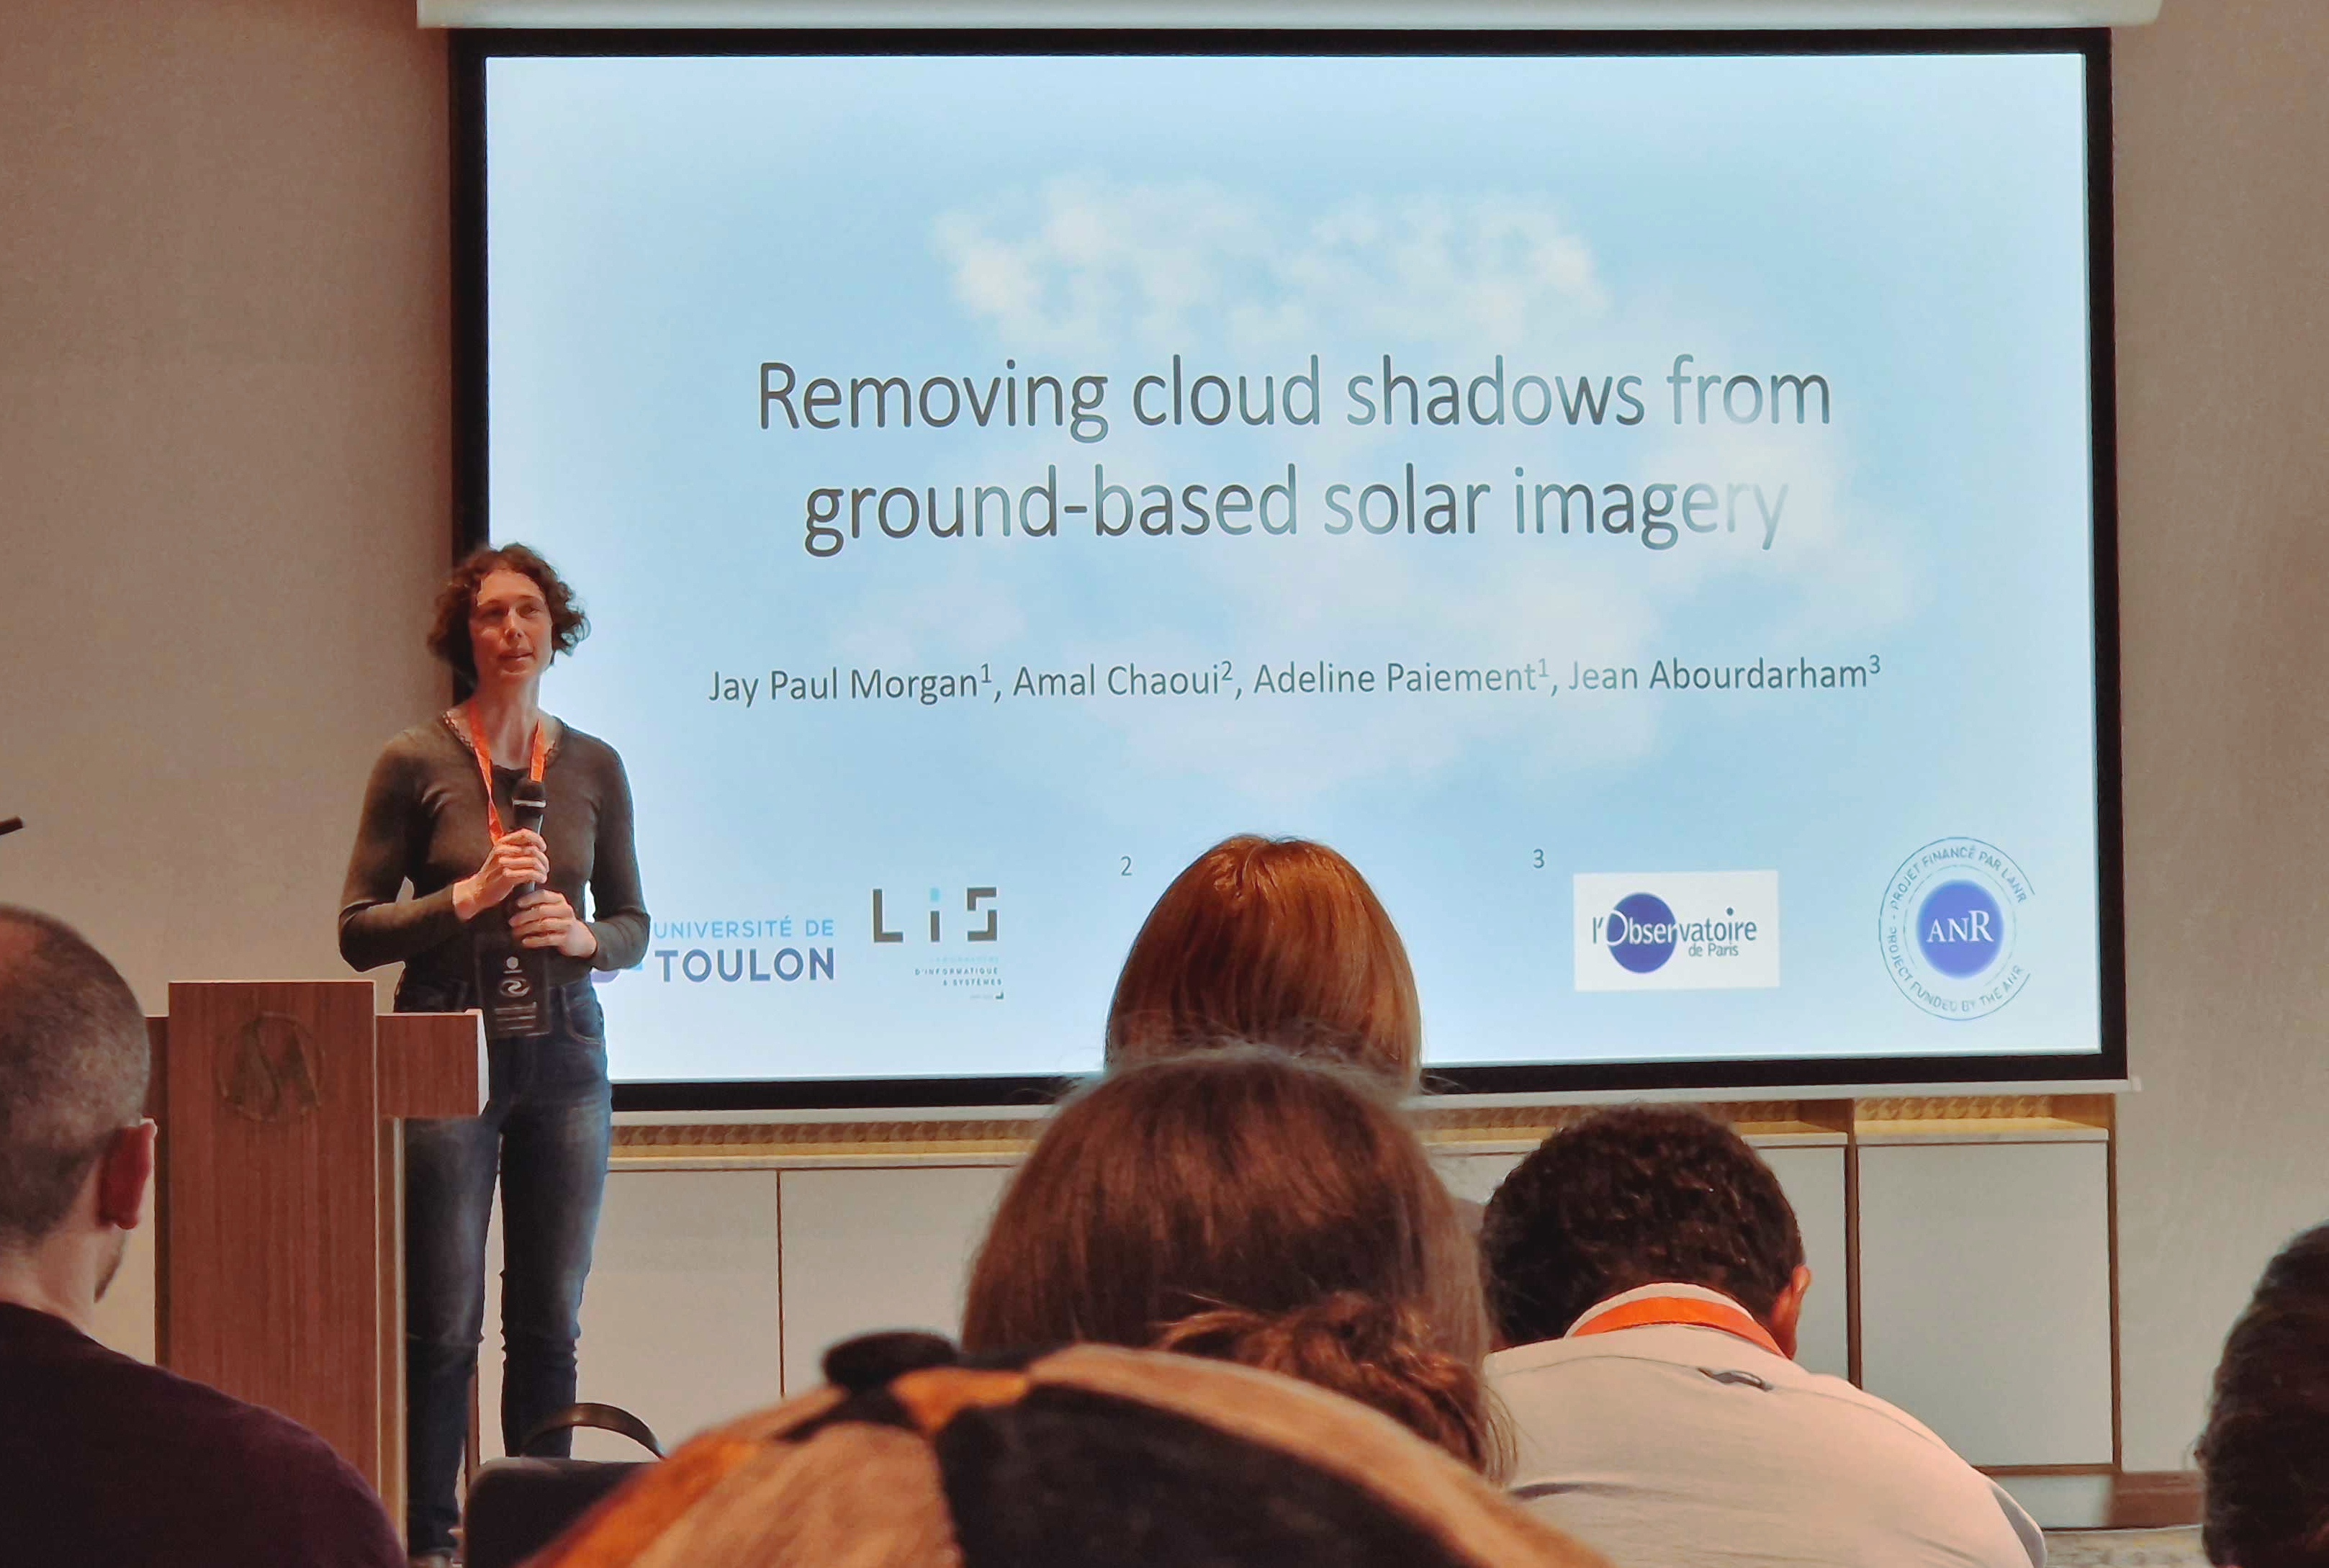
\includegraphics[width=1.0\textwidth]{images/20230420_163823.jpg}
\caption{Adeline Paiement presenting our working on removing cloud shadows from ground-based imaging.}
\end{figure}

Adeline Paiement presented our work on the cleaning of cloud
contaminants from H-\(\alpha\) and Ca-II imaging. We used a U-Net model in
a C-GAN architecture to learn the cloud transmittance. The
transmittance values could then be added to the solar disk, resulting
in a cleaned image.



, up-scaling of existing data, cleaning and
pre-processing.

\section{Other talks}
\label{sec:orgff30e68}

\begin{figure}[htbp]
\centering
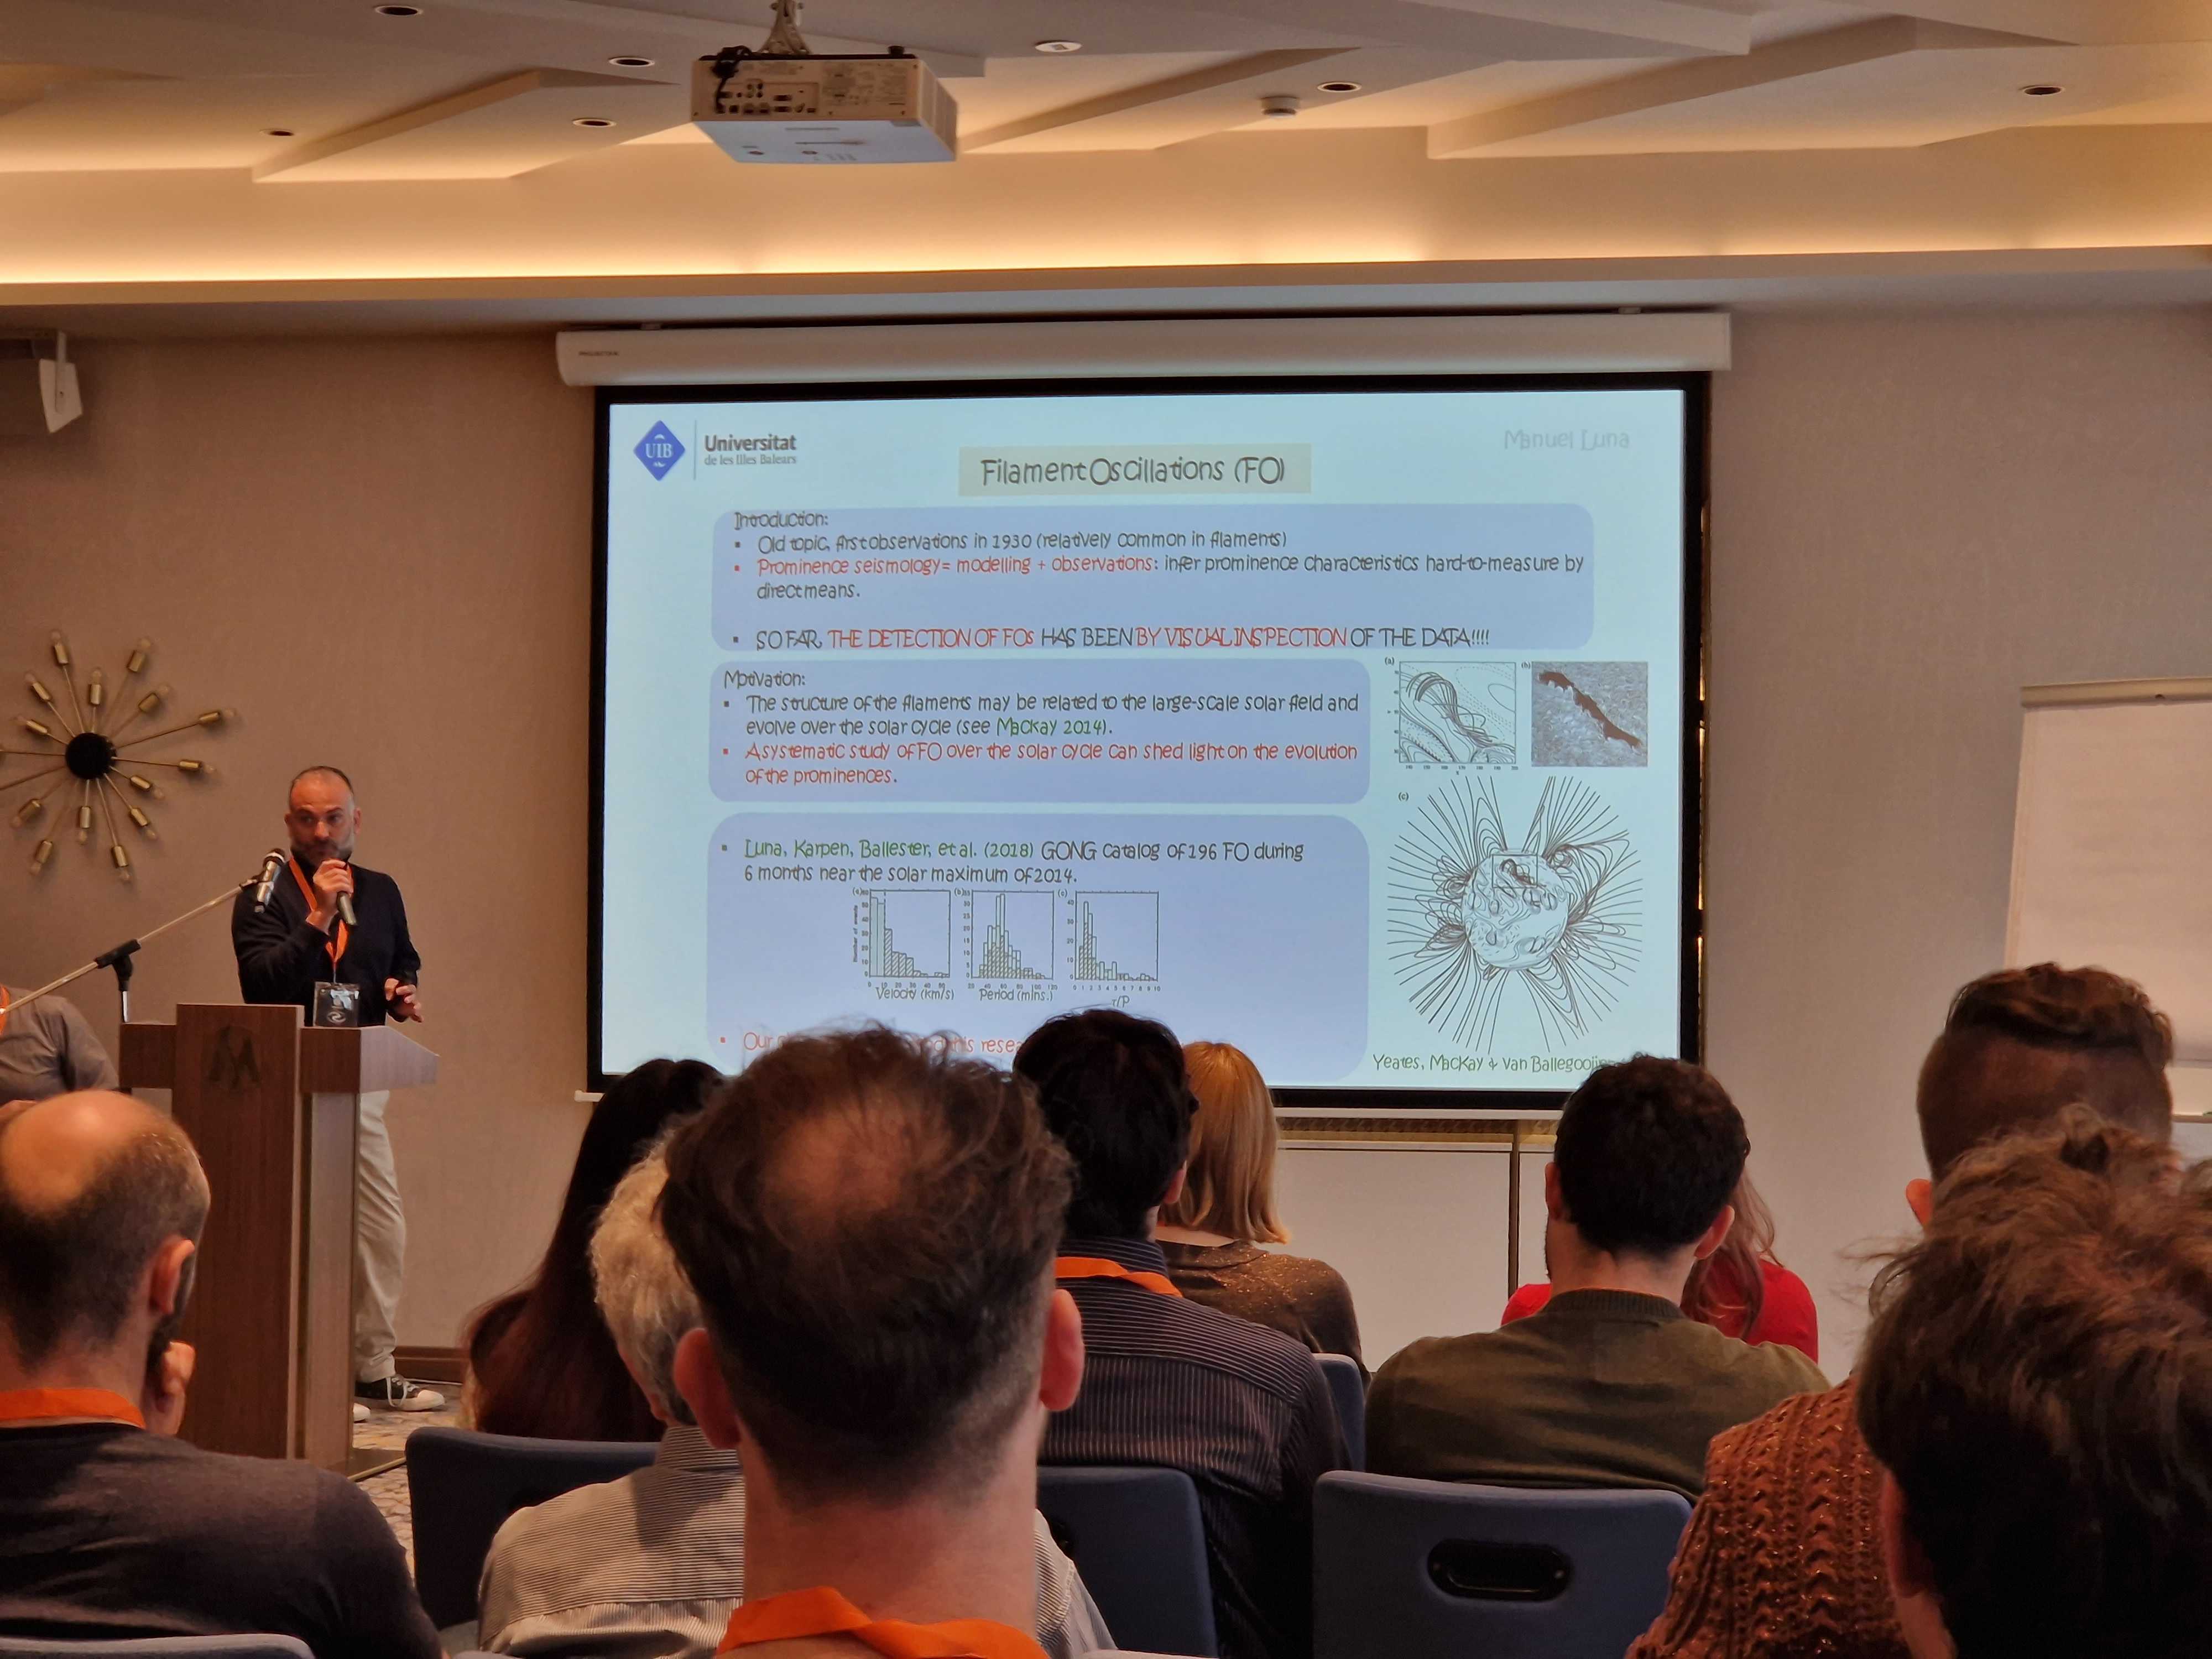
\includegraphics[width=1.0\textwidth]{images/20230419_102413.jpg}
\caption{Manuel Luna presenting his work on the characterisation on the oscillisation of filaments.}
\end{figure}

Not all of the talks fit into my classification here. But I wanted to
highlight some other interesting talks that do not follow the trend
placed above, though this in itself is not an exhaustive list. First
we have Manuel Luna's work of detecting the oscillation of filament
structures and its characterisation over a 6-month period. Secondlly,
we have Benoit's talk of creating a 3d-simulation of the sun by
predicting the image of the solar disk from angles where there are no
satellites. Other works include Connor O'briens lecture on the
probabilisitc determination of solar wind propagation using an RNN
model

\begin{figure}[htbp]
\centering
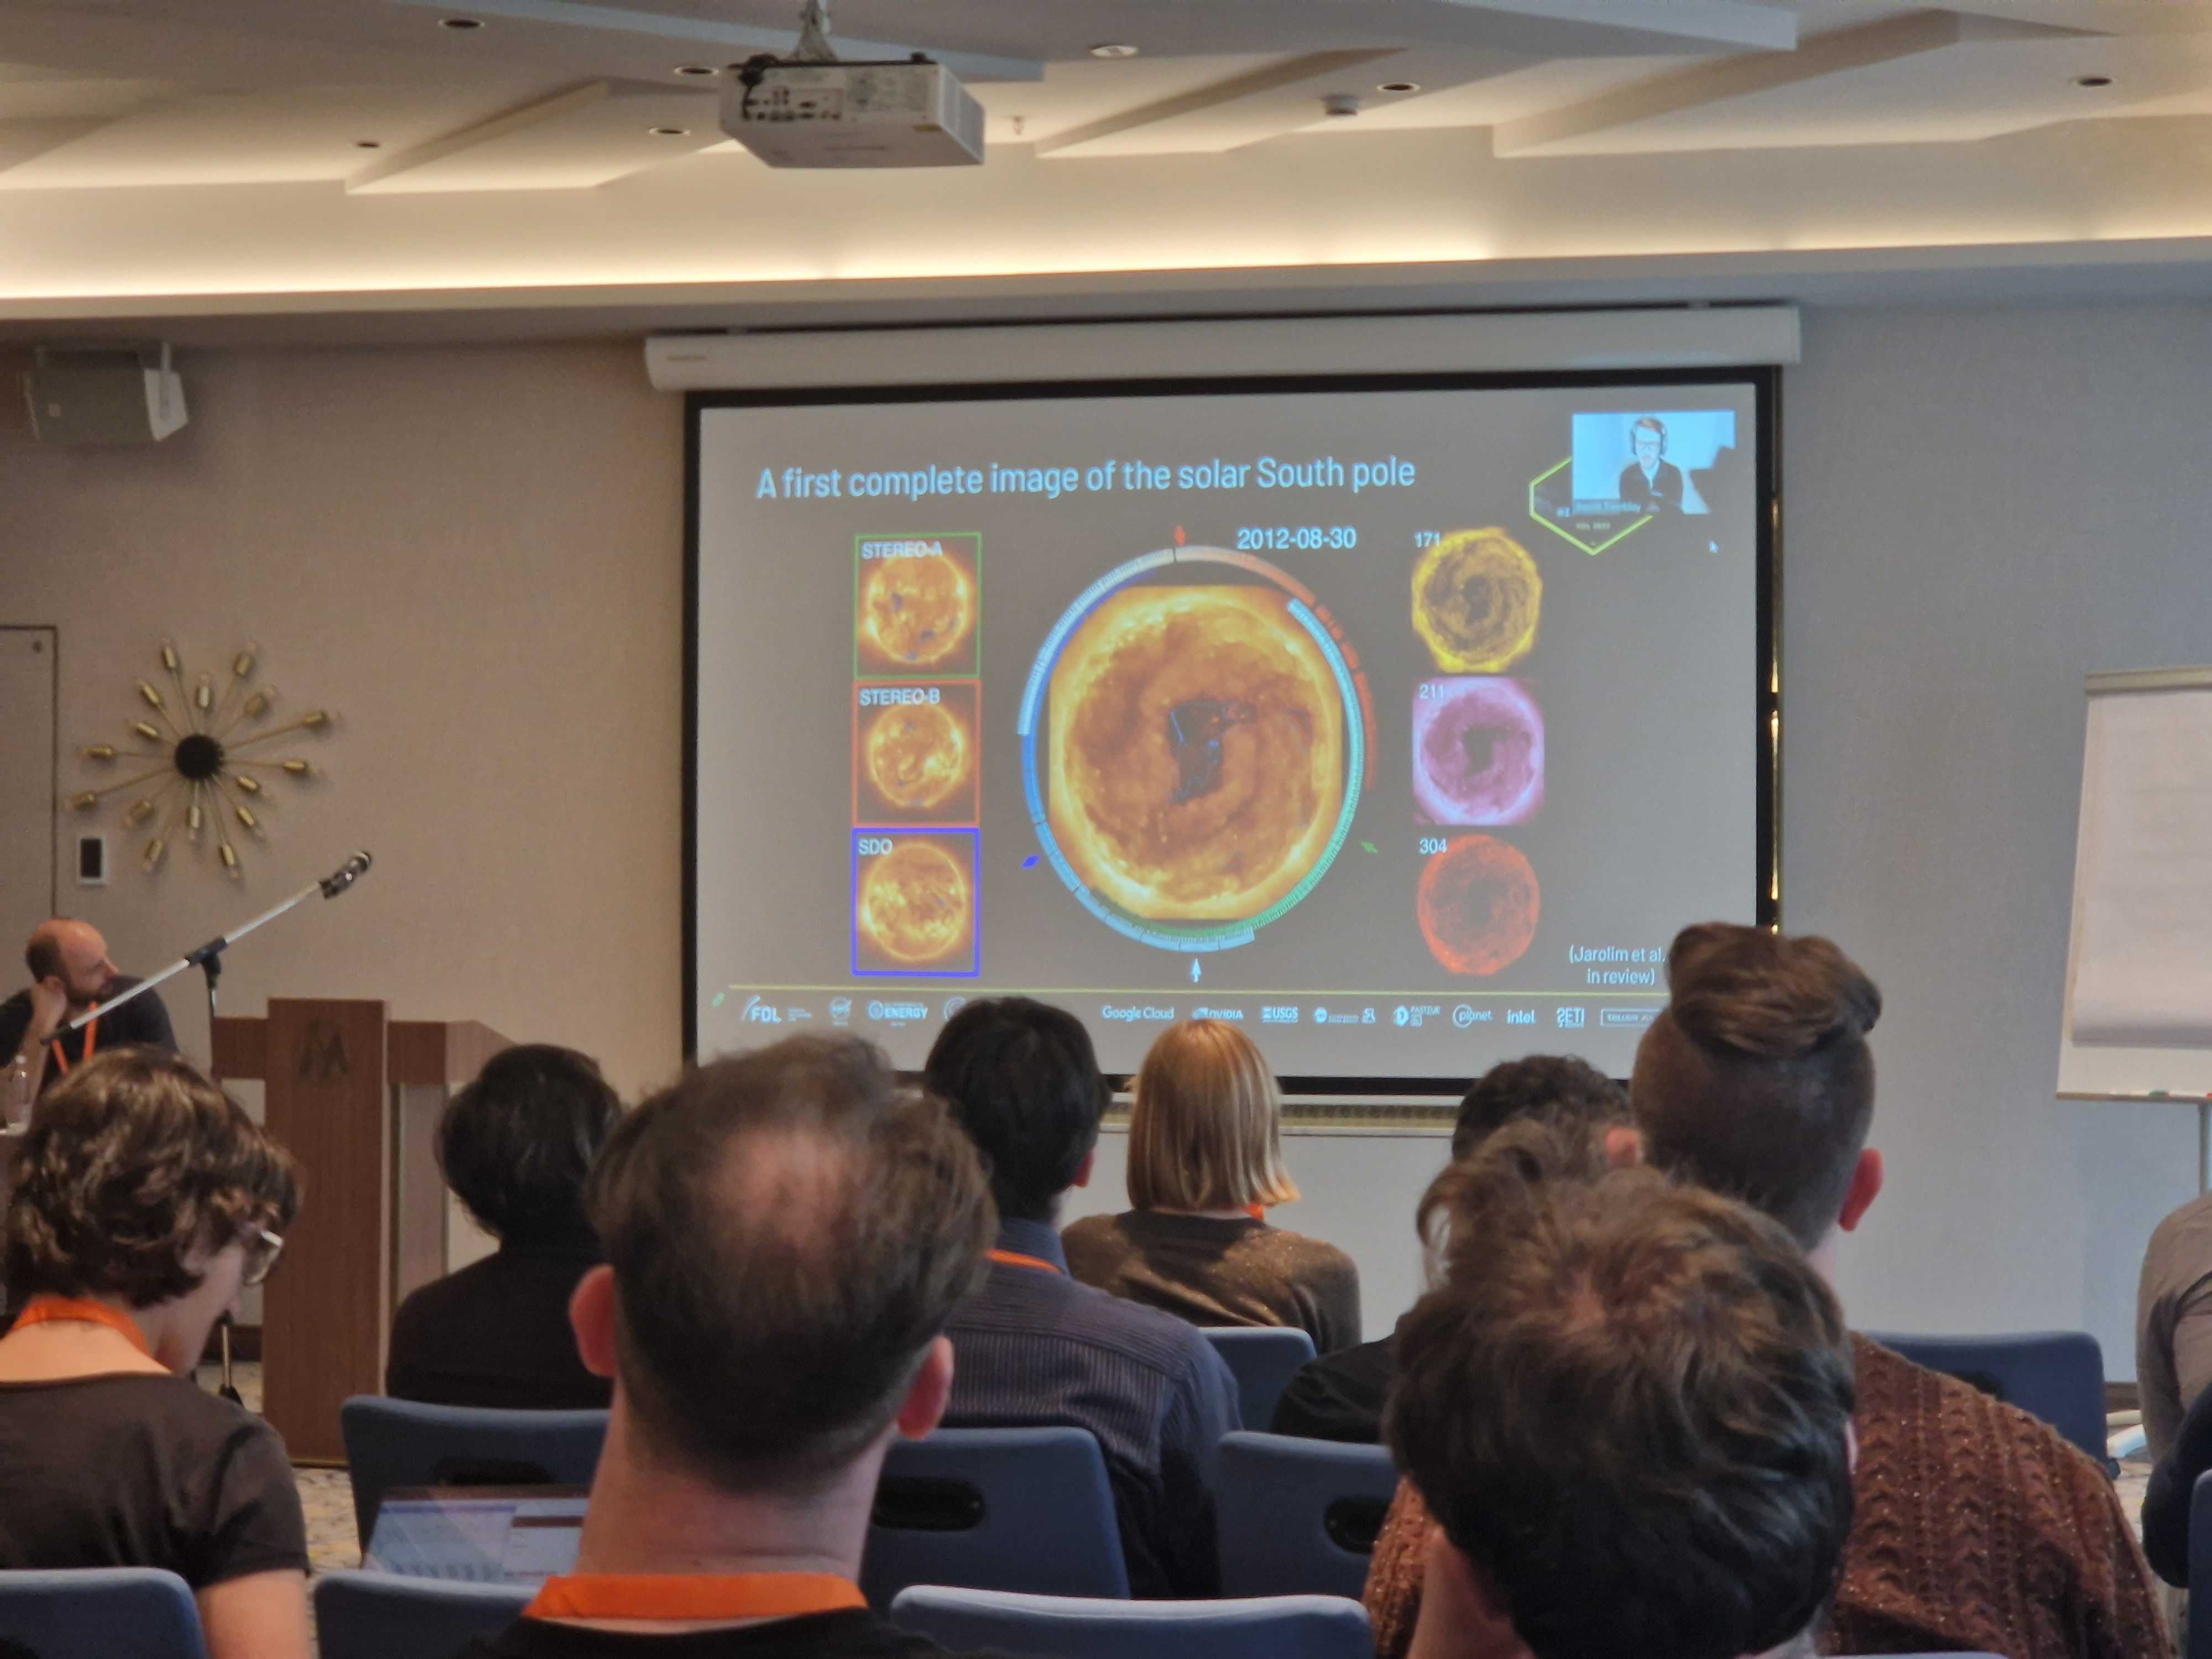
\includegraphics[width=1.0\textwidth]{images/20230419_173438.jpg}
\caption{Benoit demonstrating an example of a 3d-simulation of the Sun's south pole.}
\end{figure}

\section{A word on Sofia, Bulgaria}
\label{sec:orgfd6c064}

\begin{center}
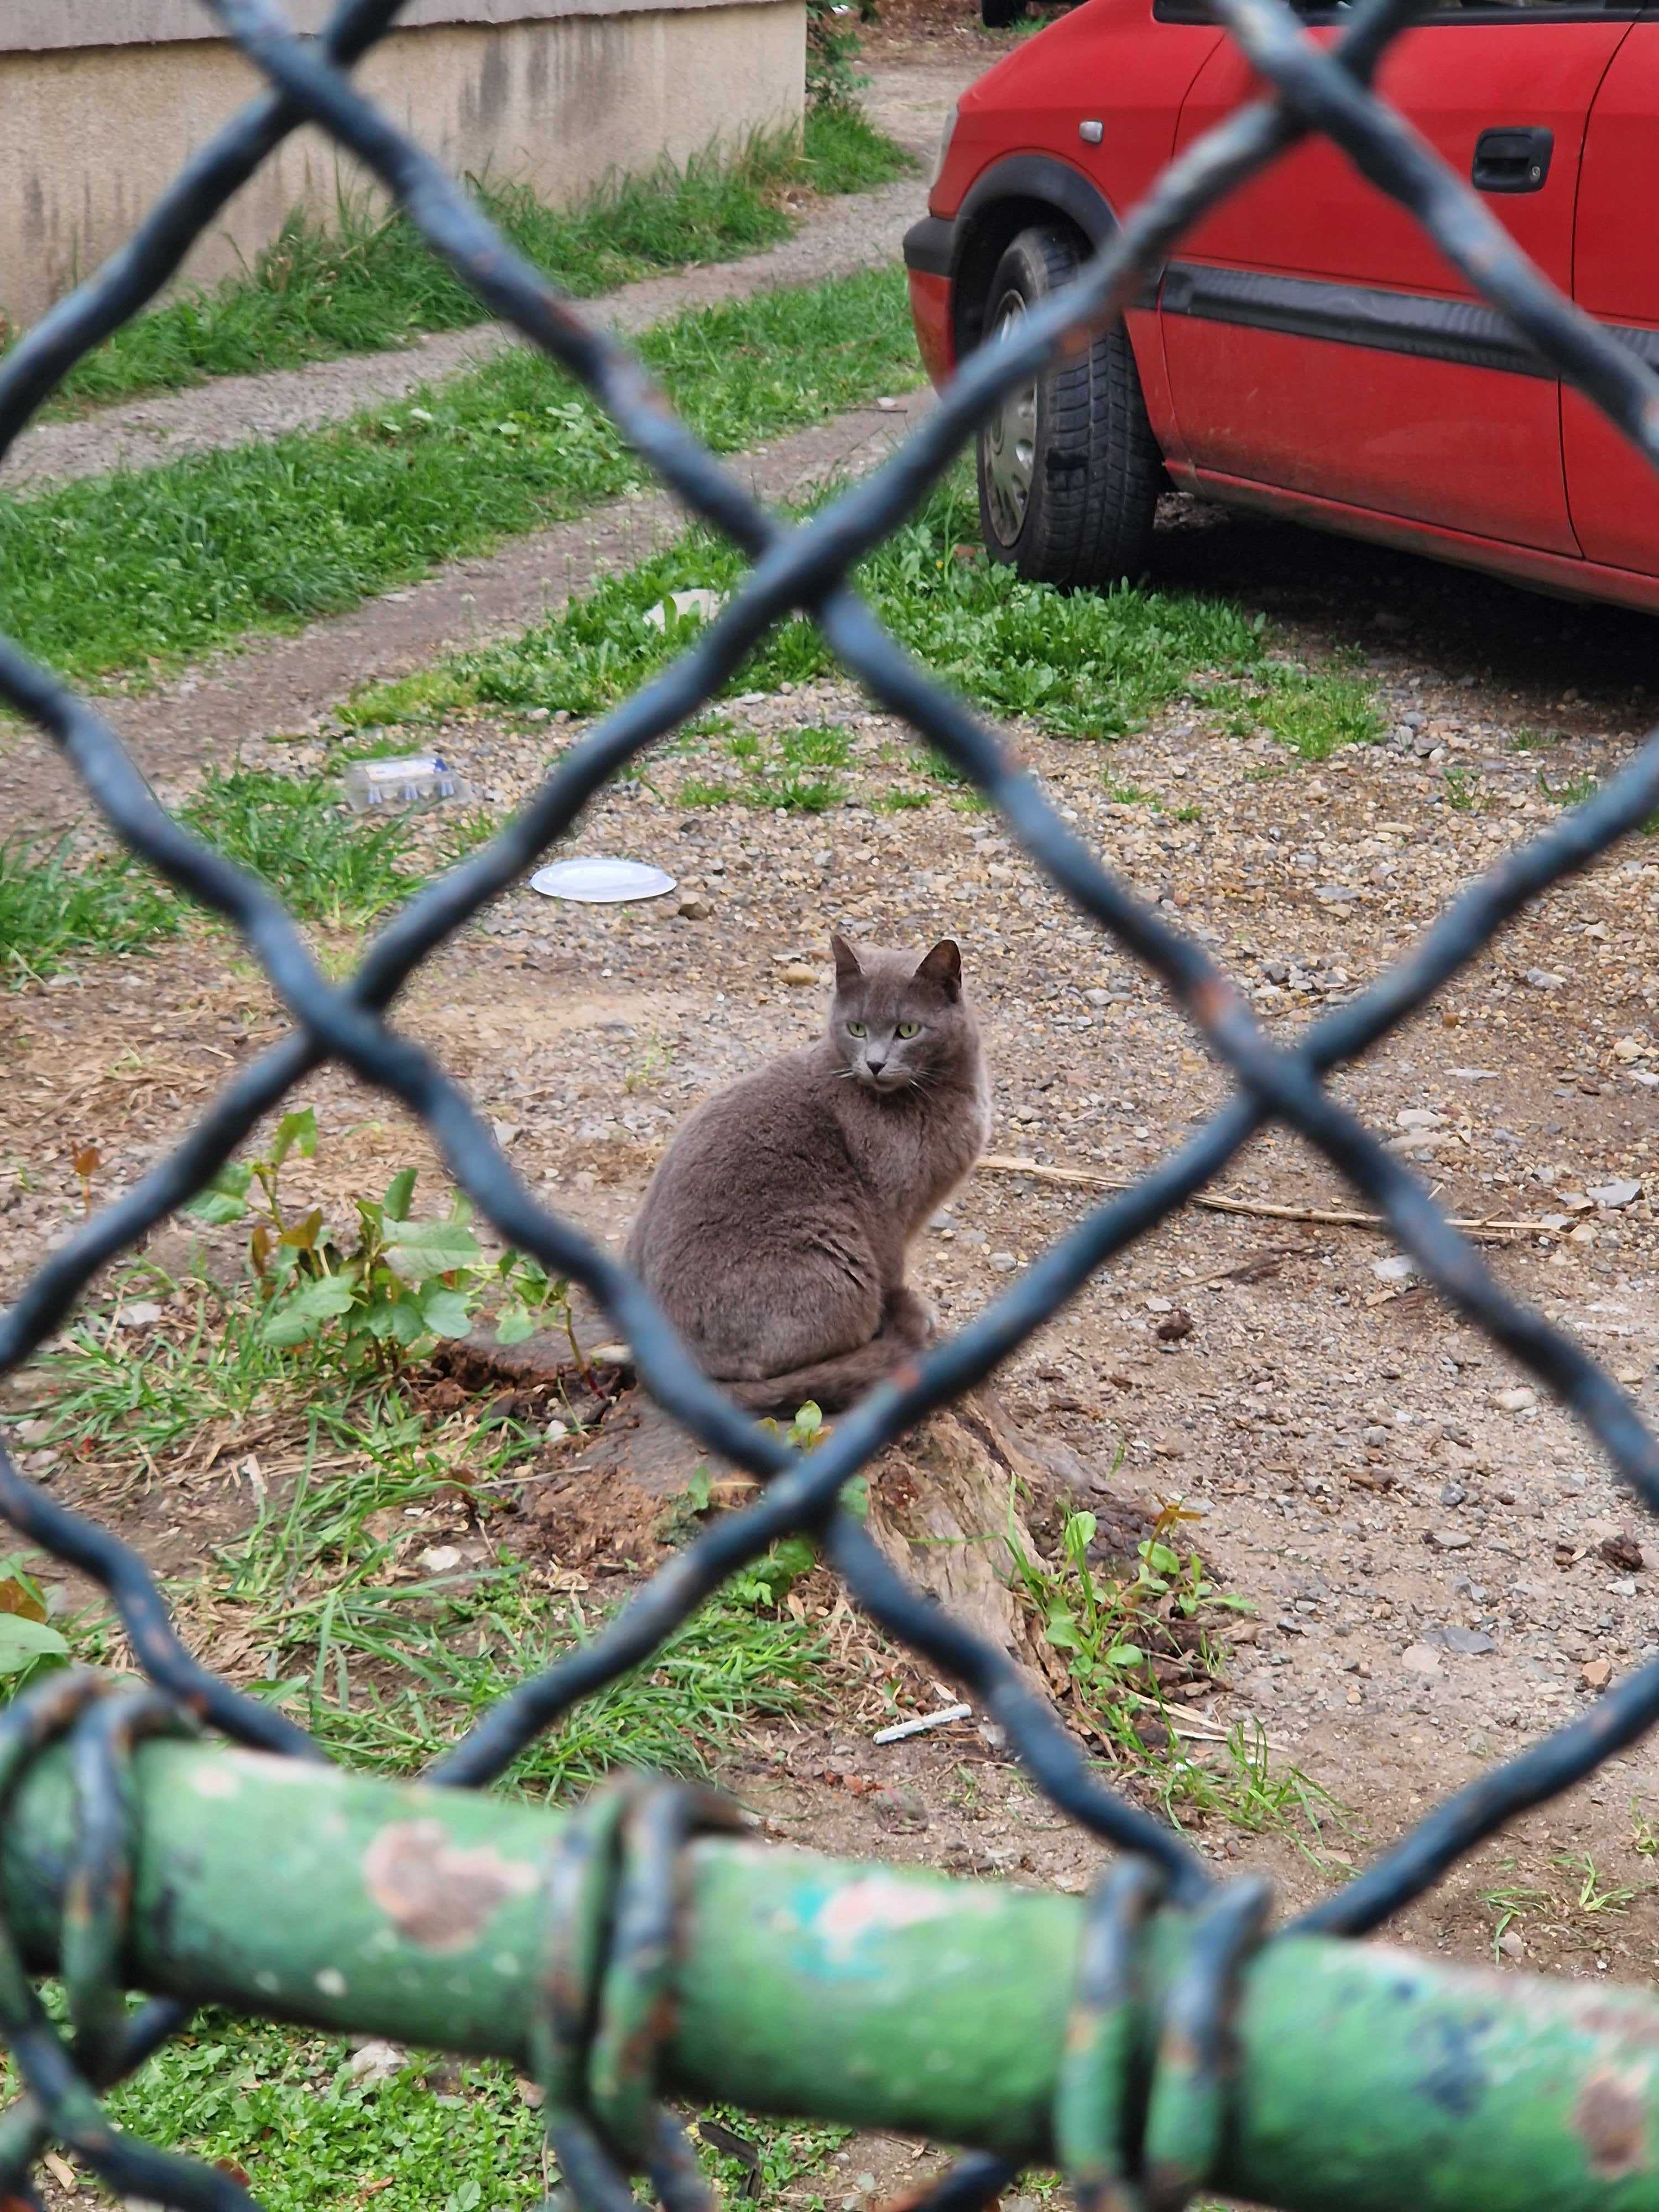
\includegraphics[width=0.5\textwidth]{images/20230421_084129.jpg}
\end{center}

\begin{center}
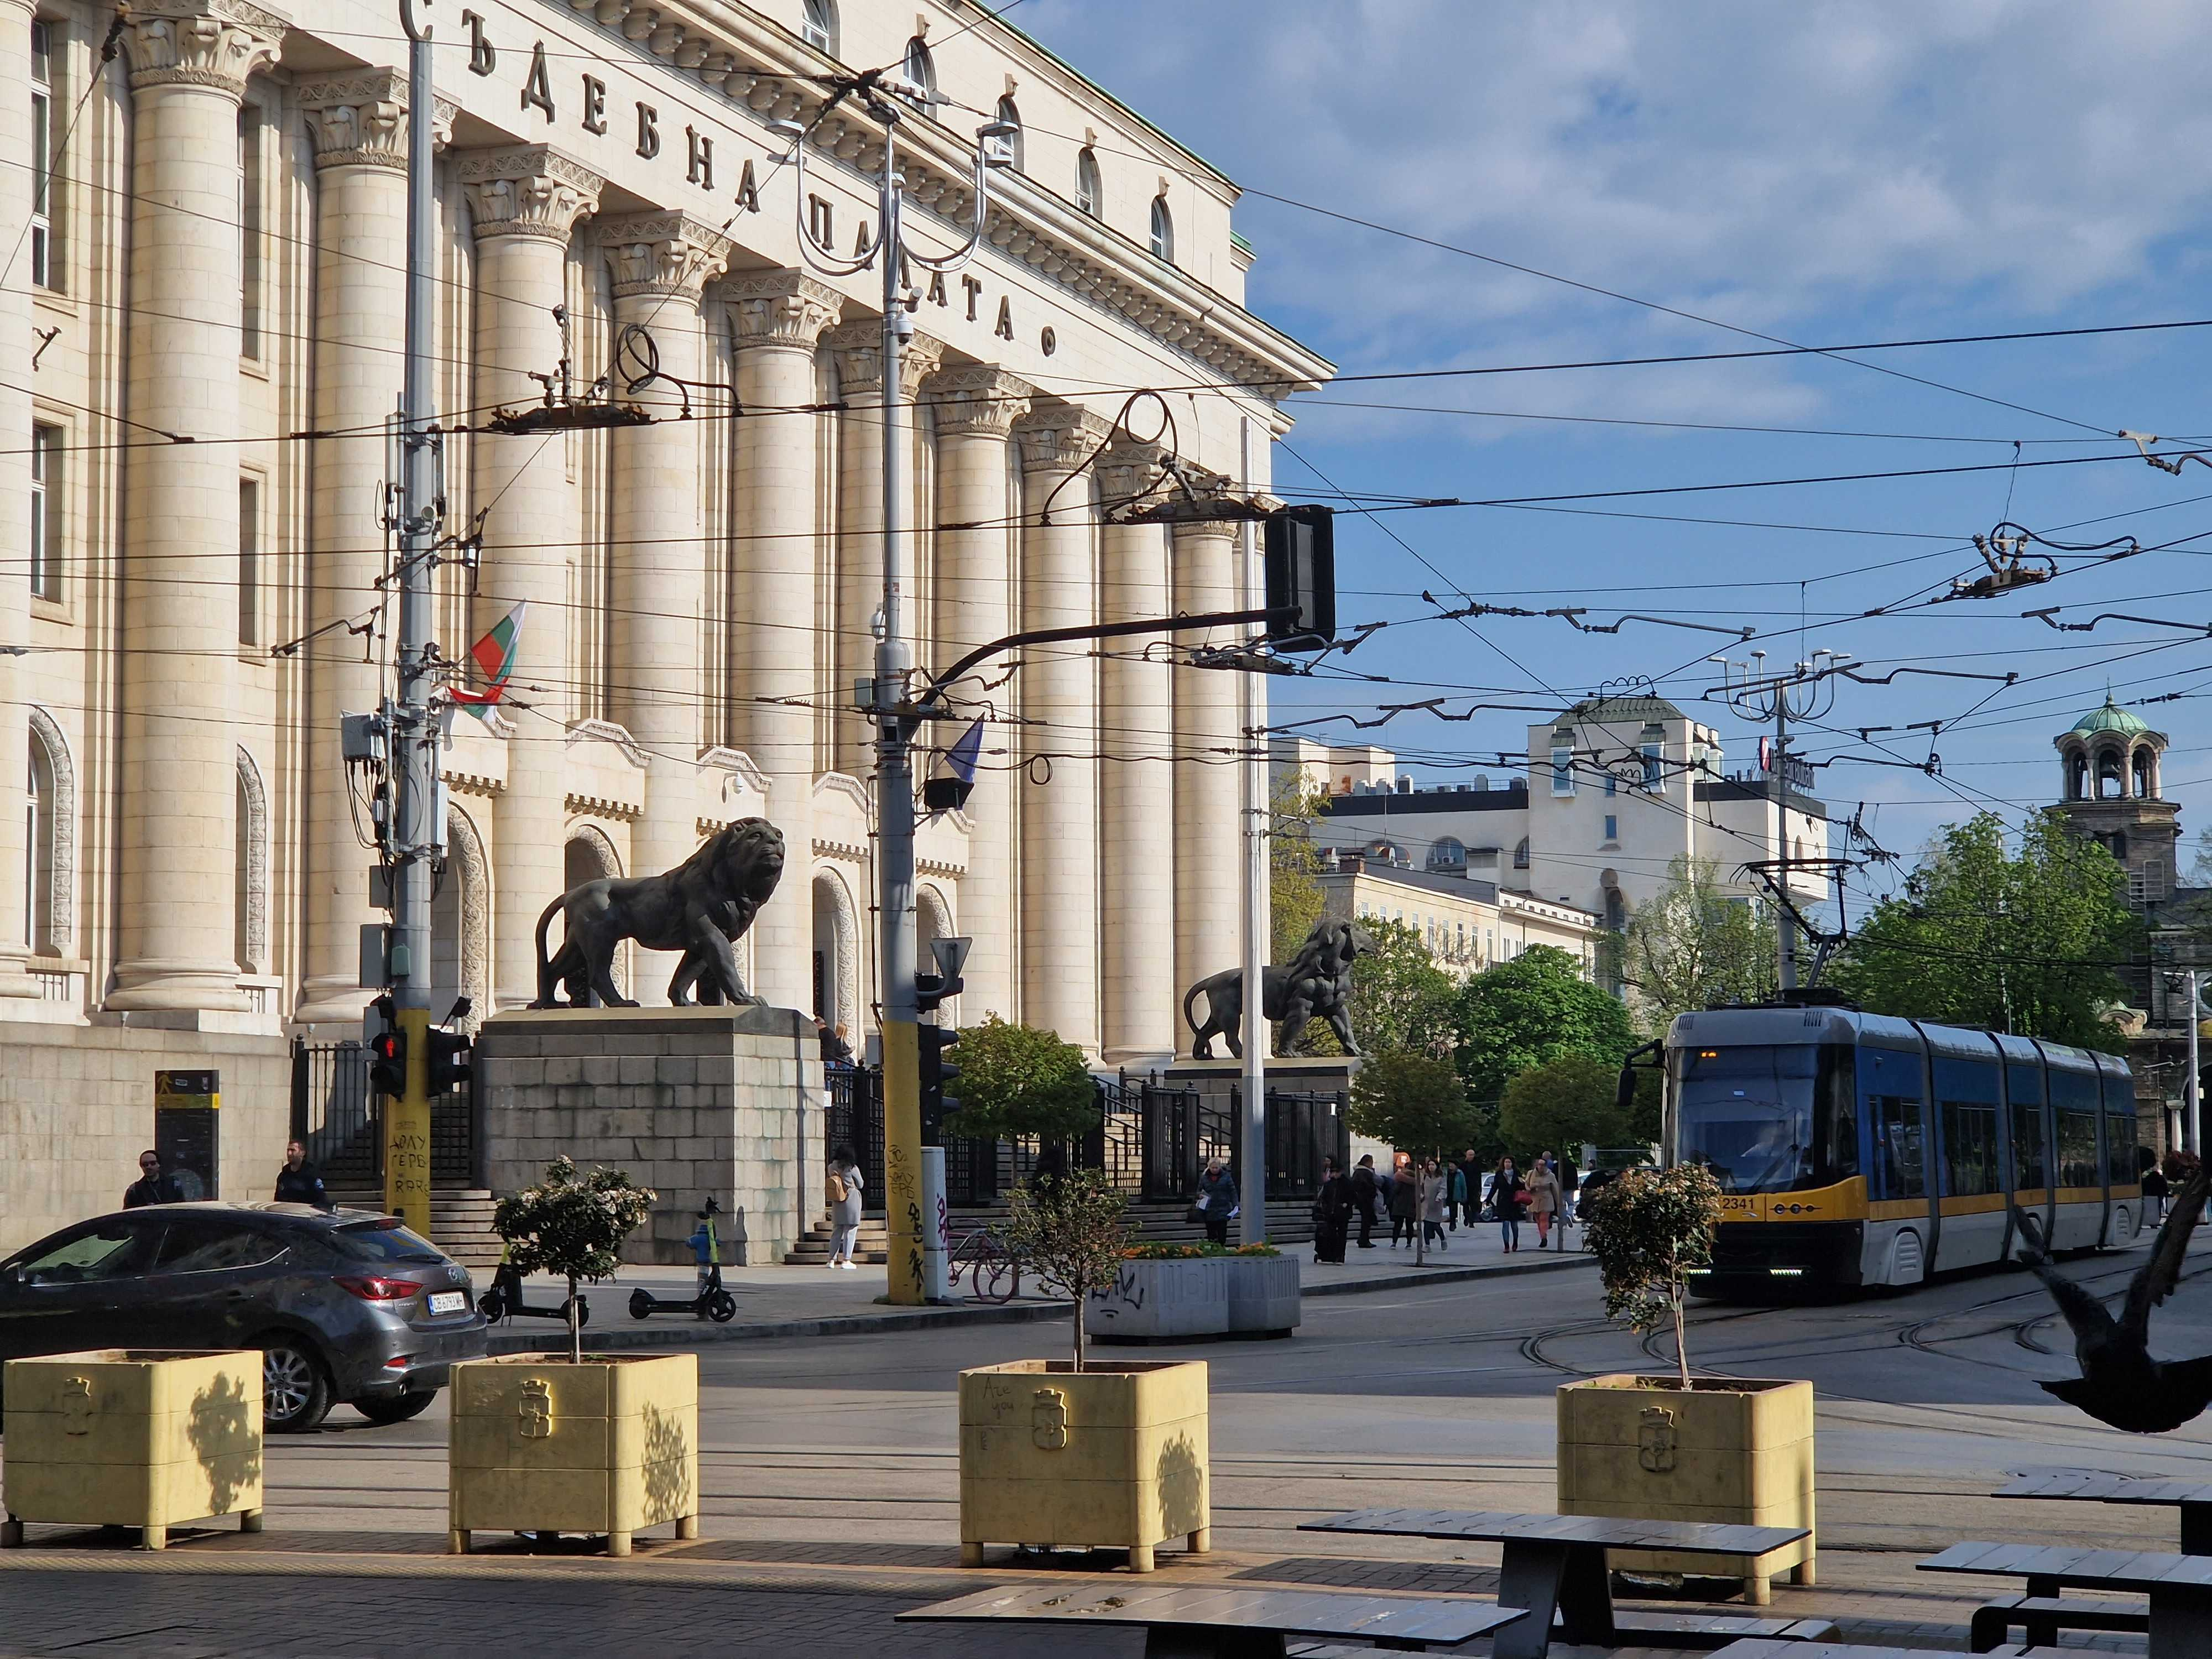
\includegraphics[width=1.0\textwidth]{images/20230421_092159.jpg}
\end{center}

\begin{center}
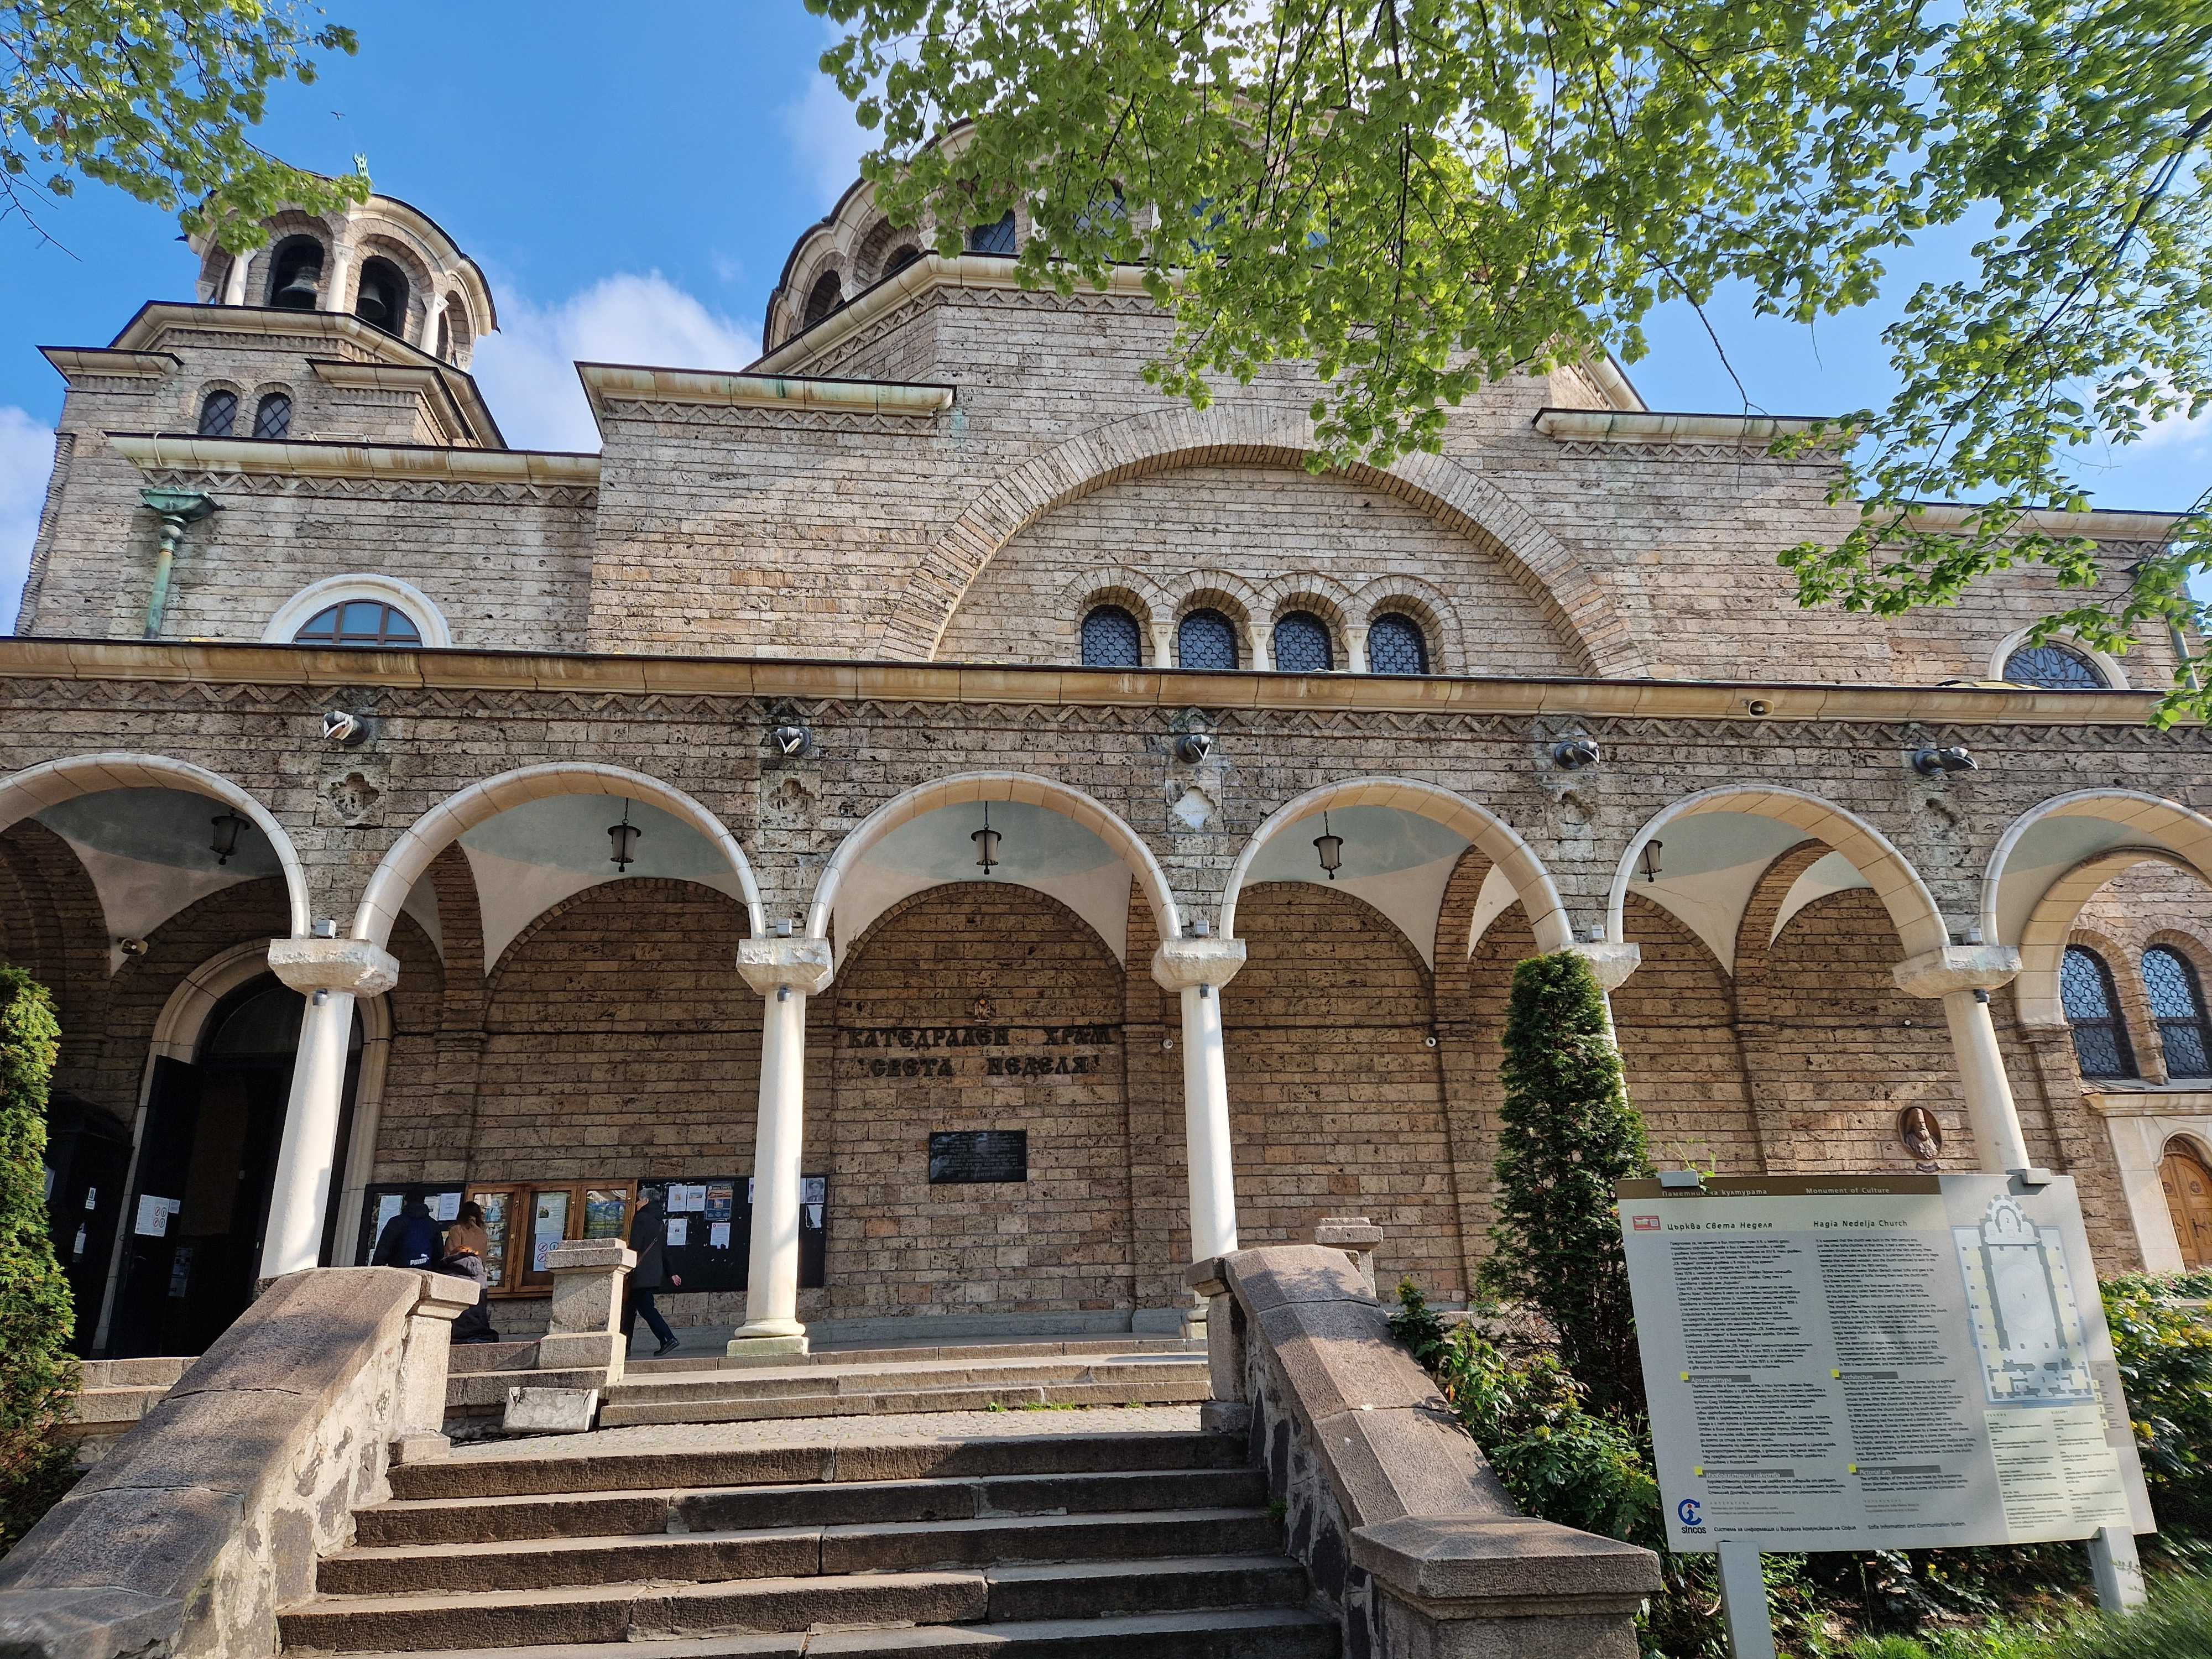
\includegraphics[width=1.0\textwidth]{images/20230421_092428.jpg}
\end{center}

\begin{center}
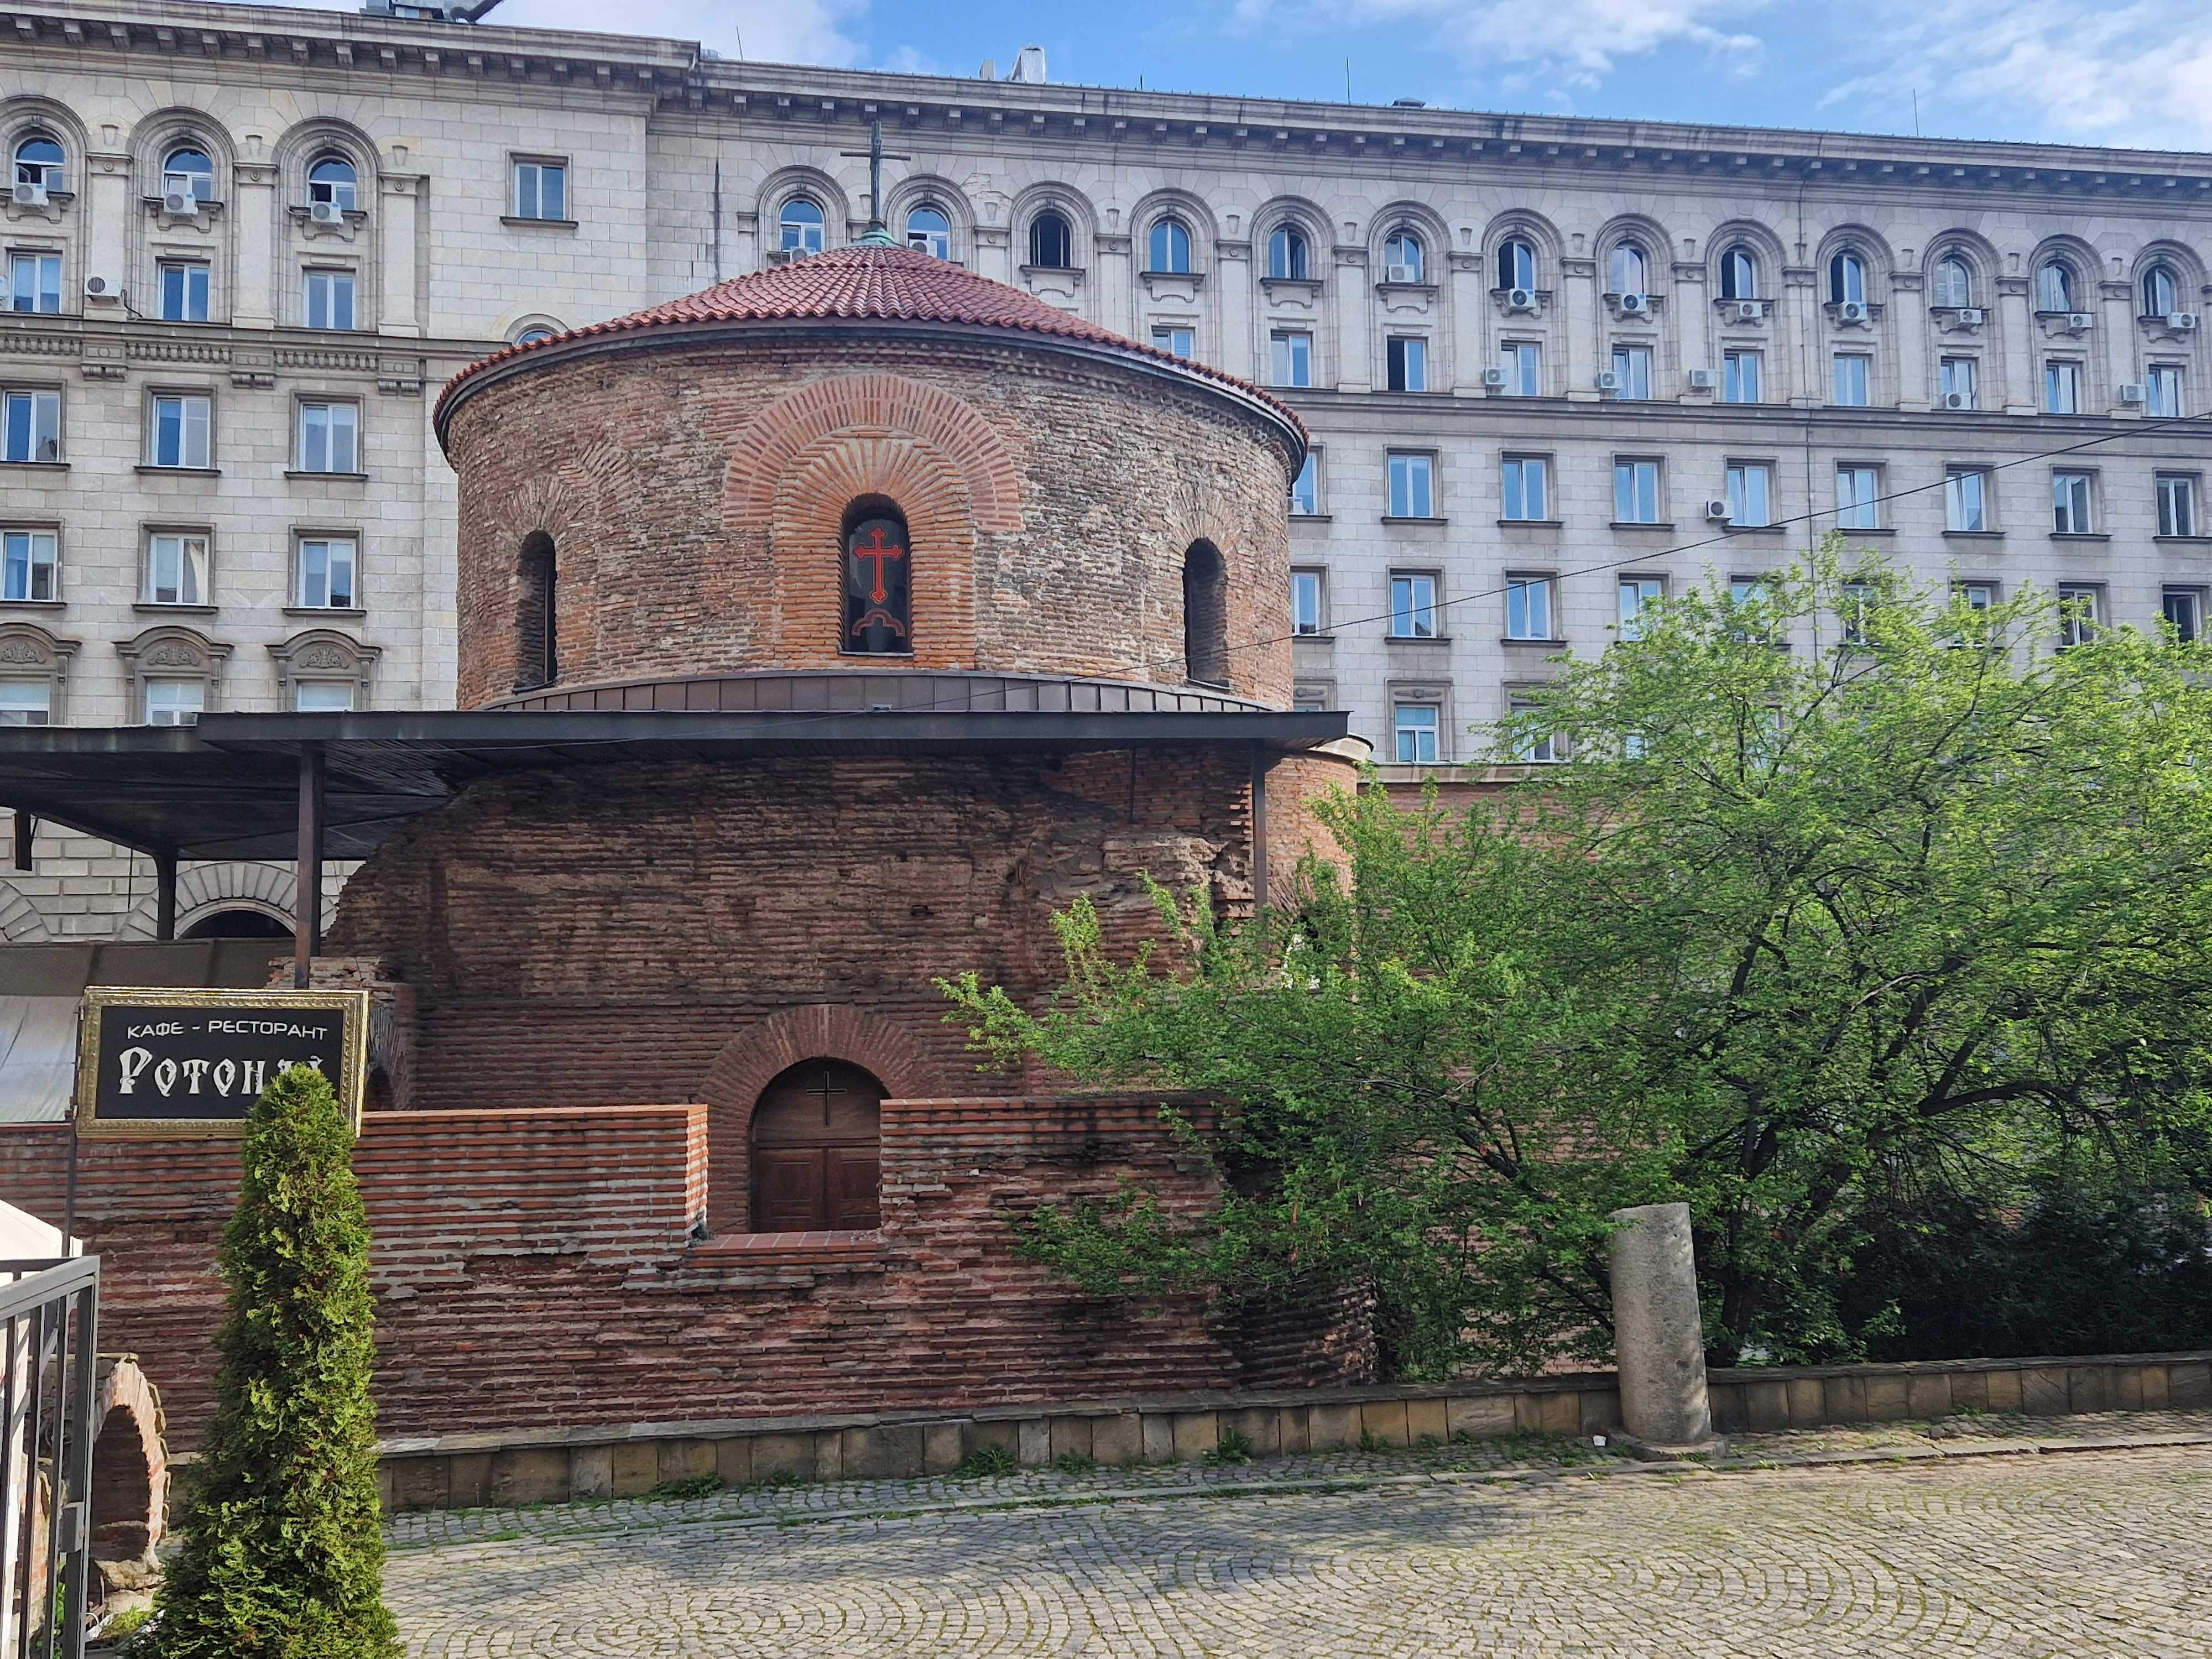
\includegraphics[width=1.0\textwidth]{images/20230421_092737.jpg}
\end{center}

\begin{center}
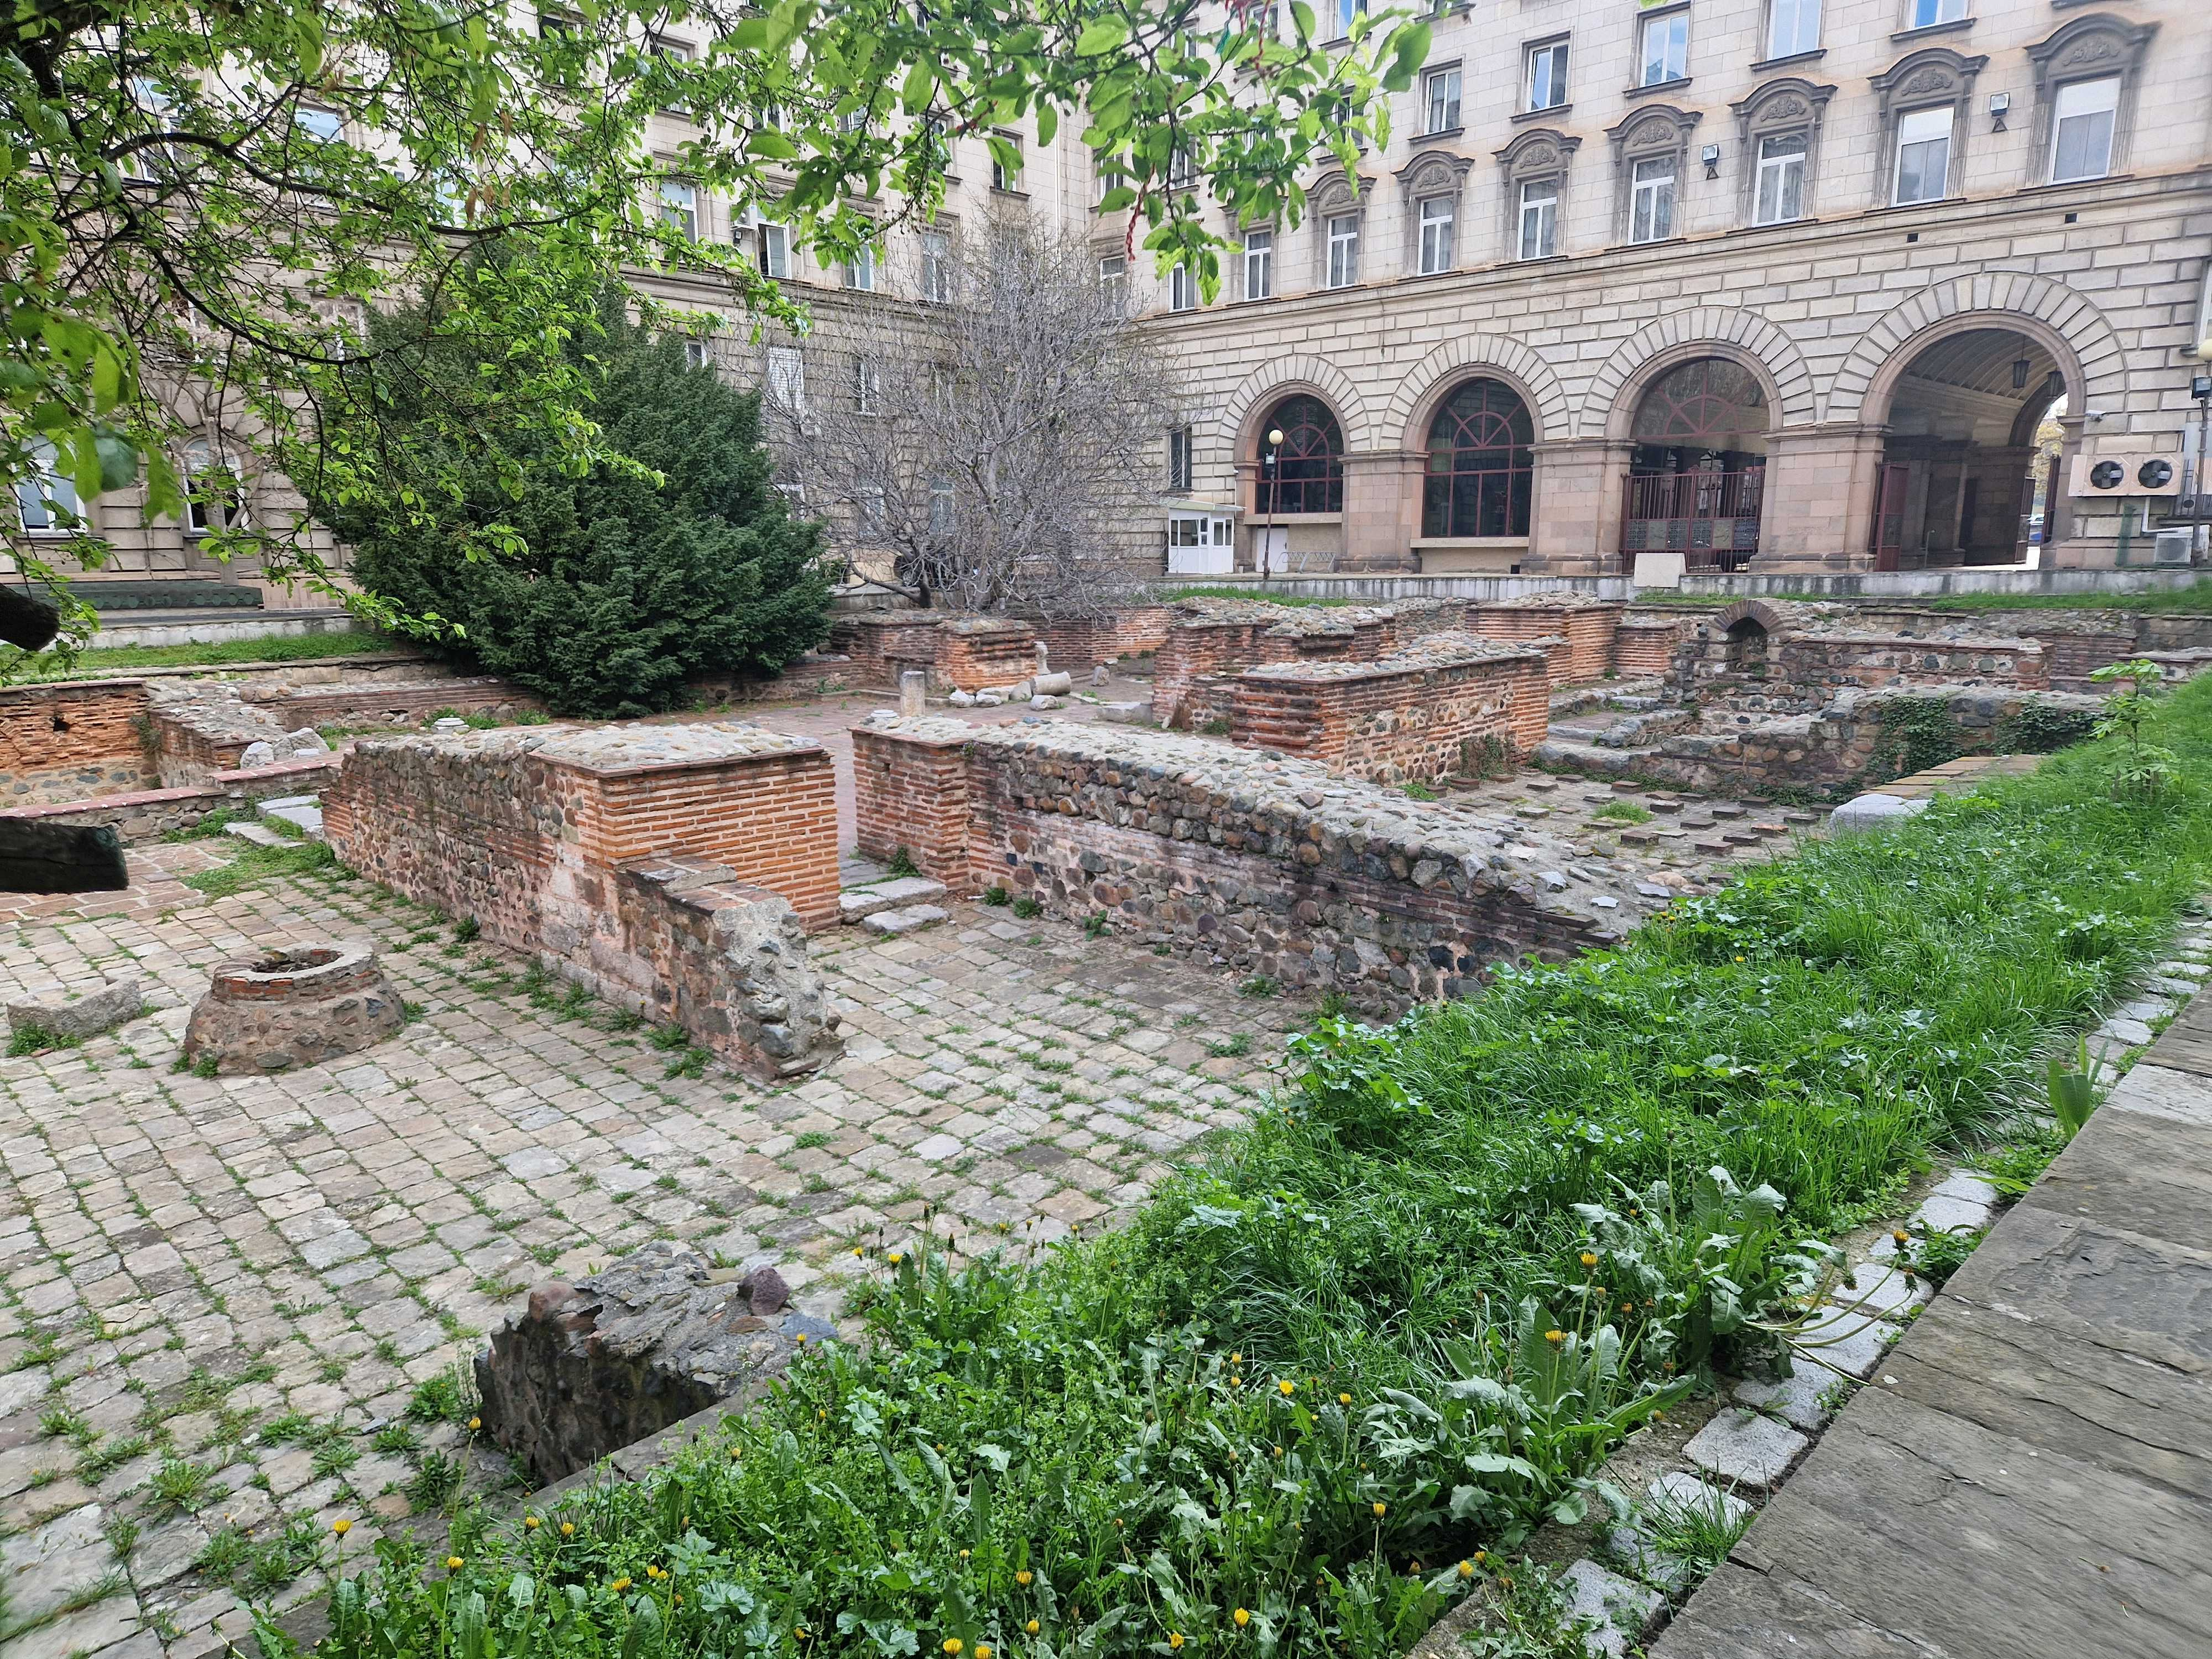
\includegraphics[width=1.0\textwidth]{images/20230421_092814.jpg}
\end{center}

\begin{center}
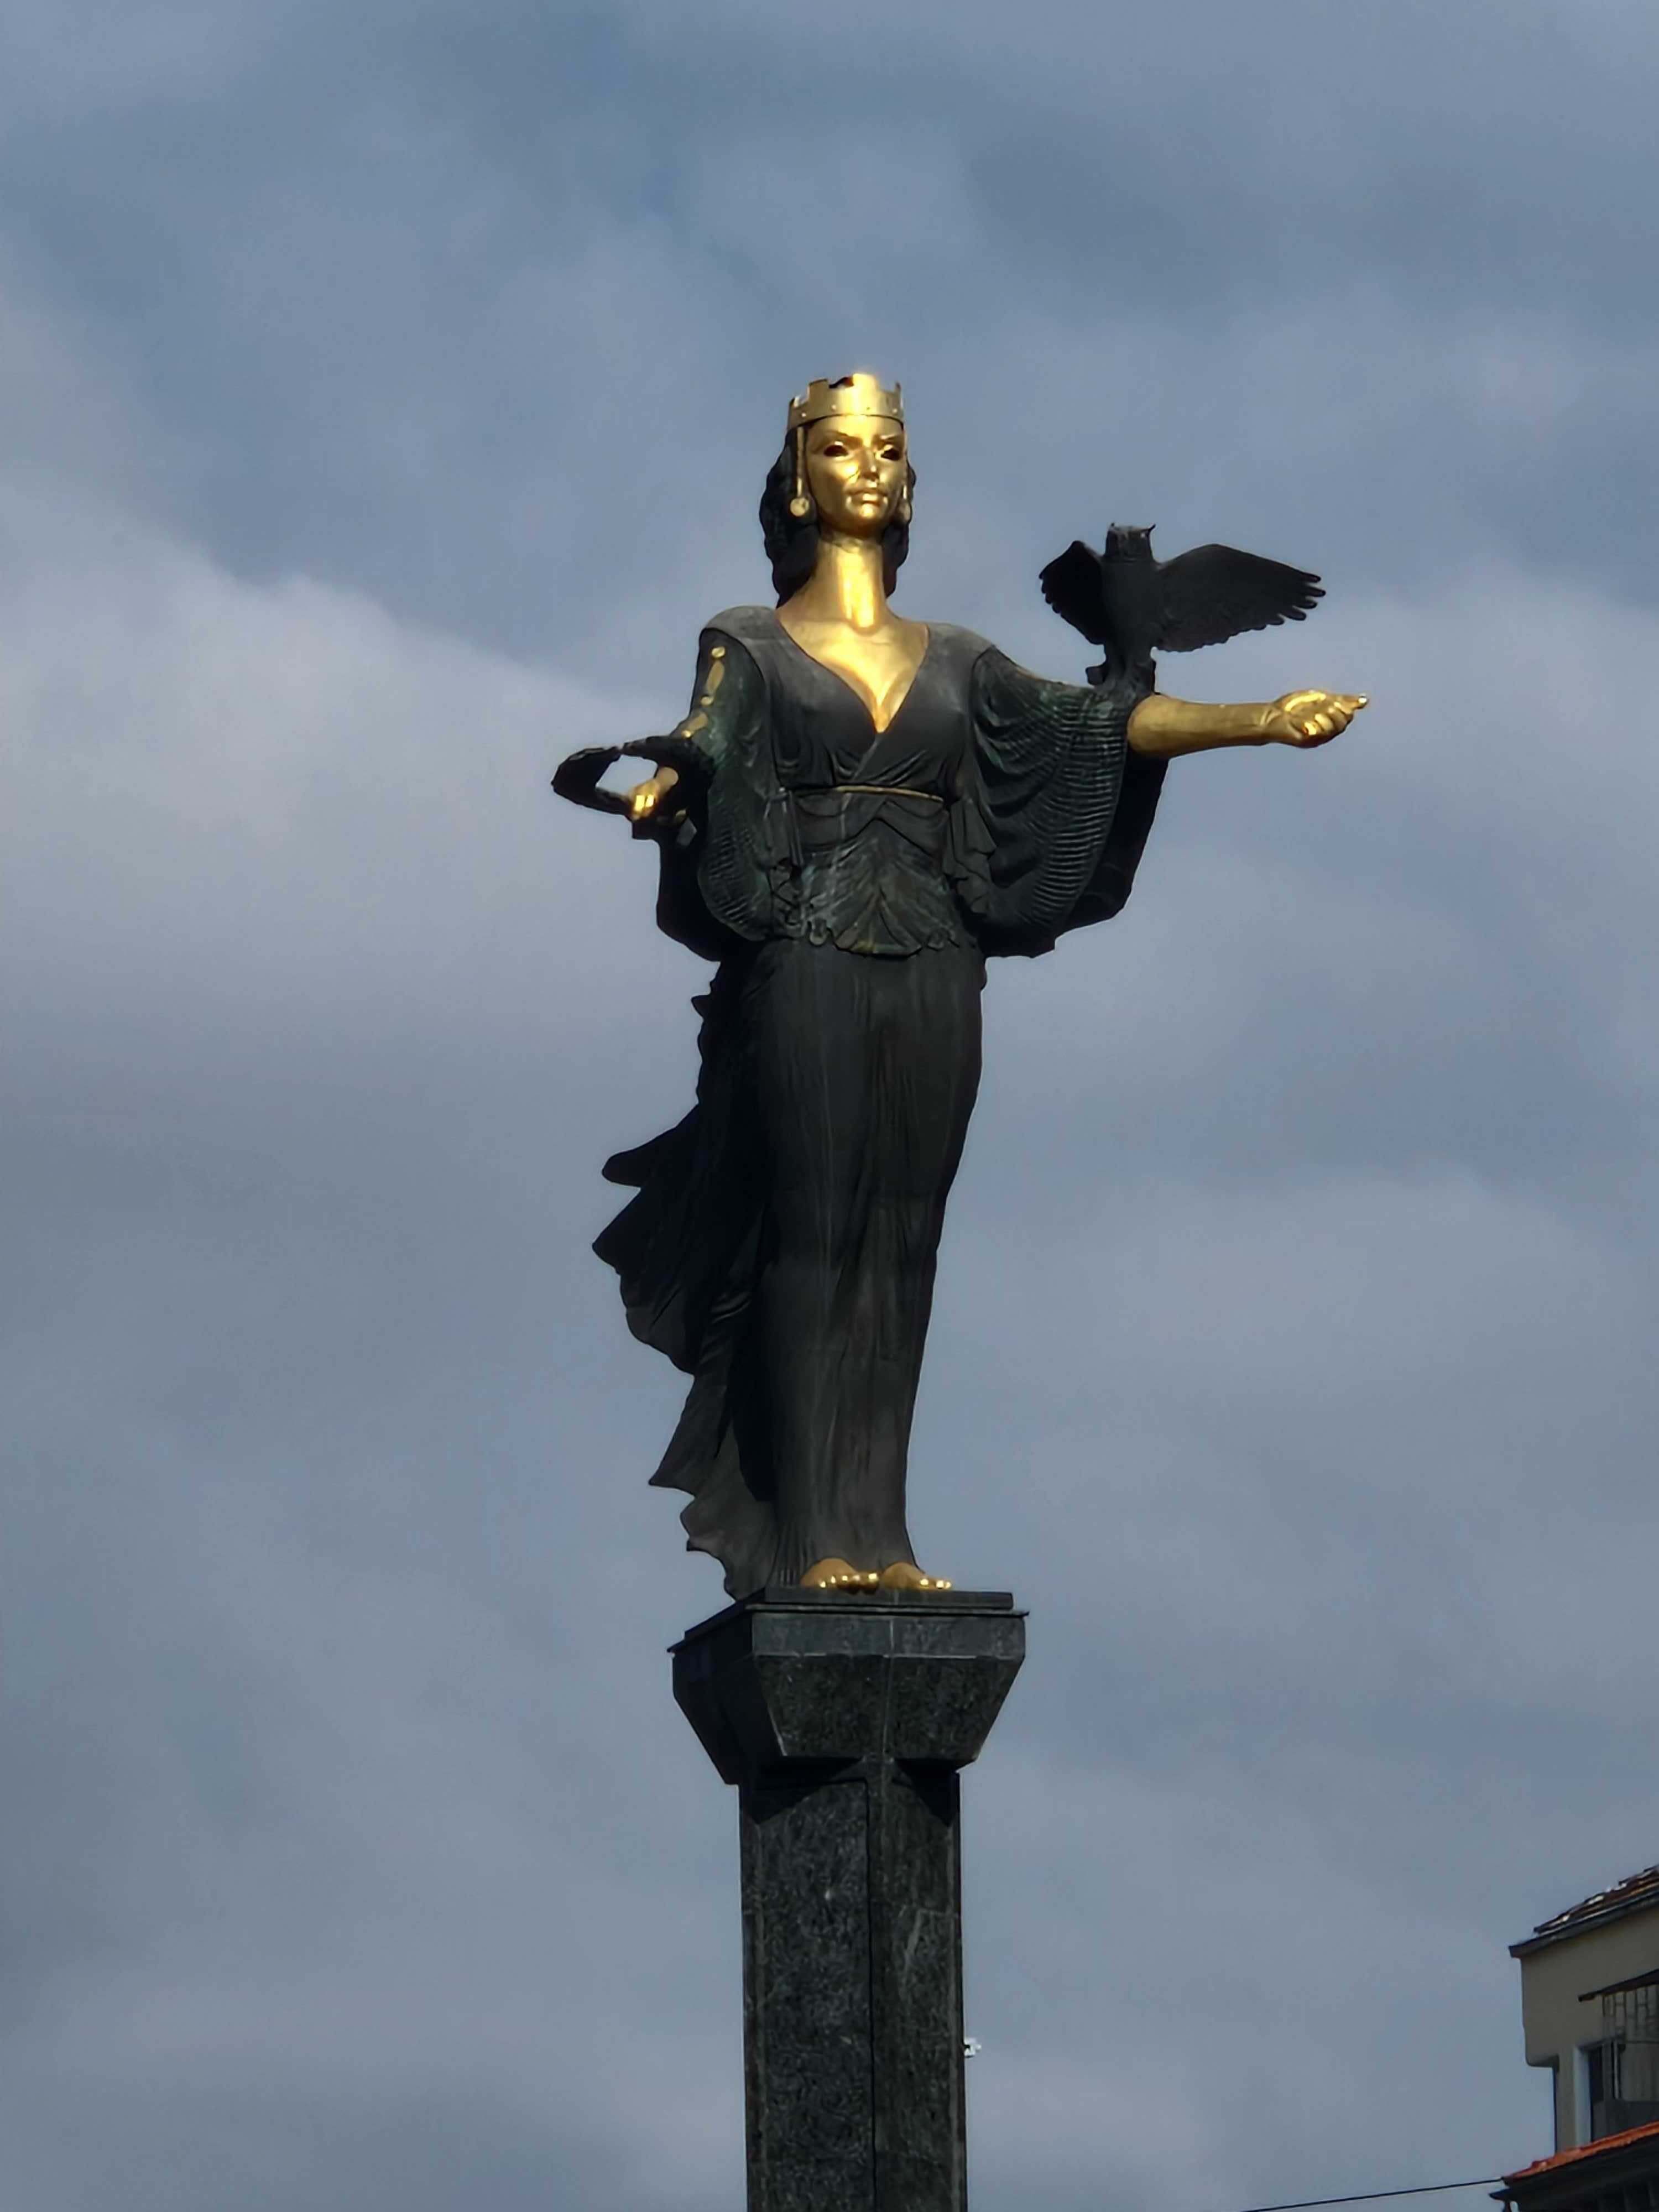
\includegraphics[width=0.5\textwidth]{images/20230421_093521.jpg}
\end{center}
\end{document}